\documentclass[10pt,twoside, fleqn]{memoir}
%\usepackage{createspace}
%\usepackage[size=pocket,noicc]{createspace}
%\usepackage[paperwidth=4.25in, paperght=6.875in,bindingoffset=.75in]{geometry}
\usepackage[T1]{fontenc}
\usepackage{mathpazo} % USE PALATINO FONT
%\usepackage{newpxtext,newpxmath}
\usepackage[latin1]{inputenc}
%\usepackage[xindy]{imakeidx}
%\usepackage{imakeidx}
\usepackage[nomain,acronym,xindy,toc]{glossaries}
%\usepackage{glossaries} %For acronyms
\usepackage[british]{babel}
%\usepackage{tgtermes}
%\usepackage[framed, numbered, autolinebreaks]{mcode} %MATLAB Snippet code
\usepackage{listings}
\usepackage{graphicx}
\usepackage{glossaries}
\usepackage{hyperref} % HYPERLINKS
\usepackage[font=footnotesize]{caption}
%\usepackage[hidelinks]{hyperref}
%\usepackage{xcolor}

\usepackage{subcaption}
\usepackage{pdflscape} %Landscape pages
\usepackage{pdfpages} %Insert pdf in document
\usepackage{amsmath}
\usepackage{amssymb}
\usepackage{gensymb} %Degree sign
\usepackage{footnote} %Footnotes in tabulars
\usepackage{xcolor,framed,marginnote,blindtext}
\hypersetup{
    colorlinks,
    linkcolor={blue!50!black},
    citecolor={blue!50!black},
    urlcolor={blue!80!black}
}% Get rid of that MySpace feeling in hypelinks...
\usepackage{listings} %Include code
\usepackage{multirow}
\usepackage{datetime}

\definecolor{infobackground}{RGB}{217,237,247}
\definecolor{infoforeground}{RGB}{58,135,173}
\definecolor{infoborder}{RGB}{188,232,241}
\usepackage{environ}
\usepackage{tikz} %TO CREATE BLOCK DIAGRAMS
\usetikzlibrary{fit,backgrounds,calc}
%\usepackage{vrsion}
\colorlet{shadecolor}{blue!10}
%\usepackage[fleqn]{amsmath}
\usetikzlibrary{shapes,arrows}
\usetikzlibrary{positioning}

\setcounter{tocdepth}{2} % DEPTH OF TABLE OF CONTENTS; 2= SUBSECTIONS INCLUDED
\setcounter{secnumdepth}{2} % SUBSECTIONS ARE NUMBERED

\usepackage[clockwise, figuresright]{rotating}
\usepackage{longtable}
\usepackage{tabu}

\NewEnviron{alertinfo}[1]
{
    \begin{tikzpicture}
    \node[inner sep=0pt,
          draw=infoborder,
          line width=1.2pt,
          fill=infobackground] (box) {\parbox[t]{.99\textwidth}
        {%
            \begin{minipage}{.15\textwidth}
                \centering\tikz[scale=3]
                \node[scale=1]
                {
                    
\includegraphics[scale=0.04]{./Images/Warning.png}
                };
            \end{minipage}%
           \begin{minipage}{.80\textwidth}
                \vskip 10pt
                \textbf{\textcolor{infoforeground}{#1}}\par\smallskip
                \textcolor{infoforeground}{\BODY}
                \par\smallskip
            \end{minipage}\hfill
        }%
    };

    \end{tikzpicture}
}


%\usepackage{mathpazo}
%\usepackage[protrusion=true,expansion=true]{microtype}
%\usepackage{type1cm}
%\usepackage{lettrine}

%\checkandfixthelayout

% See the ``Memoir customise'' template for some common customisations
% Don't forget to read the Memoir manual: memman.pdf

%\title{TITLE OF BOOK}
%\author{NAME OF AUTHOR}
%\date{} % Delete this line to display the current date

%% BEGIN TITLE

\makeatletter
\def\maketitle{%
  \null
  \thispagestyle{empty}%
  \vfill
  \begin{center}\leavevmode
    \normalfont
    {\LARGE\raggedleft \@author\par}%
    \hrulefill\par
    {\huge\raggedright \@title\par}%
    \vskip 1cm
  {\Large \@date\par}%
  \end{center}%
  \vfill
  \null
  \cleardoublepage
  }
\makeatother
\author{Paolo Baesso}
\title{AIDA Trigger logic unit (TLU)}
\date{\today}
\loadglsentries{O:/LatexFiles/Glossary/myGlossary.tex}
%\input{O:/LatexFiles/Glossary/myGlossary.tex}
%\makeglossaries


%%% BEGIN DOCUMENT
\makeindex
\begin{document}

\def\brd{FMC\_TLU\_v1E }
\def\oldbrd{FMC\_TLU\_v1C }

\let\cleardoublepage\clearpage


\maketitle
\frontmatter

\null\vfill
\begin{flushleft}
\textit{Board \brd.}\newline
\newline
Paolo Baesso - \monthname,   \the\year\newline paolo.baesso@bristol.ac.uk
\bigskip

\end{flushleft}
\let\cleardoublepage\clearpage

\newpage
\tableofcontents

\mainmatter
\sloppy

\newenvironment{SpecialPar}
  {\begin{shaded}\noindent}
  {\end{shaded}}



%%% INCLUDE CHAPTERS

%\def\conn{\verb|HDMI1|}
%\def\conn{\verb|HDMI2|}
%\def\conn{\verb|HDMI3|}
%\def\conn{\verb|HDMI4|}
%\include{ch_Introduction}




\chapter{Introduction}\label{ch:introduction}
This manual describes the AIDA \gls{tlu} designed for the \href{http://aida2020.web.cern.ch/}{AIDA-2020 project} by David Cussans\footnote{University of Bristol, Particle Physics group} and Paolo Baesso\footnote{University of Bristol, Particle Physics group}.\\
The unit is designed to be used in High Energy Physics beam-tests and provides a simple and flexible interface for fast timing and triggering signals at the AIDA pixel sensor beam-telescope.\\
The current version of the hardware is an evolution of the \href{https://twiki.cern.ch/twiki/bin/view/MimosaTelescope/TLU}{EUDET-TLU} and the \href{https://www.ohwr.org/projects/fmc-mtlu/wiki}{miniTLU} and is shipped in a metallic case that includes an \gls{fpga} board and the \gls{tlu} \gls{pcb}: the \gls{fpga} is responsible for all the logic functions of the unit, while the \gls{pcb} contains the clock chip, discriminator and interface blocks needed to communicate with other devices.\\
The current version of the \gls{pcb} is \brd and is designed to plug onto a carrier \gls{fpga} board like any other \gls{fmc} mezzanine board, although its form factor does not comply with the ANSI-VITA-57-1 standard.\\

\section{FPGA}
The \gls{tlu} is shipped with an \gls{fpga} board already programmed with the latest version of the firmware needed to operate the unit.\\
The firmware developed at University of Bristol is targeted to work with the Enclustra  AX3 board, which must be plugged onto a PM3 base, also produced by \href{http://www.enclustra.com/en/home/}{Enclustra}. The firmware is written on the \gls{fpga} using a \gls{jtag} interface. Typically a breakout board will be required to connect the Xilinx programming cable to the Enclustra PM3. All these components are included in the \gls{tlu} enclosure so the user can upload a new version of the firmware by simply connecting a \gls{usb}-B cable in the back panel of the unit.\\
At the time of writing this work\footnote{Oct 2017} the AX3 is the only \gls{fpga} for which a firmware has been developed. However, we plan to ship future versions of the \gls{tlu} with a custom made \gls{fpga} designed by Samer Kilani.
\begin{alertinfo}{Note}
    If the \gls{fpga} detects a programming cable connected it will not load the firmware from its memory after a power cycle.\\
    It is recommended to leave the \gls{usb} cable disconnected from the back panel unless there is the intention to re-program the firmware.
\end{alertinfo}


\section{Power}
The \gls{tlu} requires 12~V to operate. Power can be provided using the circular jack on the back panel of the unit.\\
During normal operation the current drawn by the unit is about 0.5~A.
%\section{Preparation}
%Before powering the \gls{tlu} it is necessary to follow a few steps to ensure the board and the \gls{fpga} work correctly.\\
%
%Currently, it is recommended to use the following:
%\begin{itemize}
% \item MA-PM3-W-R5: Mars PM3 base board
% \item MA-AX3-35-1I-D8-R3: Marx AX3 module (hosts a Xilinx XC7A35T-1CSG324I )
% \item MA-PM3-ACC-BASE: Accessory kit, including a \gls{jtag} breakout board to connect Xilinx programming cables. Also includes a 12~V power supply to power the PM3.
%\end{itemize}
%
%\section{I/O voltage setting}
%The I/O pins of the PM3 can be configured to operate at 2.5~V or 3.3~V; the factory default is 2.5~V but the \brd requires 3.3~V logic. The user should make sure to select the appropriate voltage by operating on DIP-switch CFG-A/S1200 (pin 1 set to ON).\\For reference, a top view of the board is provided in the appendix at page~\pageref{ch:appendix}.\\
%\begin{alertinfo}{Warning}
%    Please double check the PM3 board manual for the correct way to change the I/O voltage setting. Enclustra has been changing their hardware recently.
%\end{alertinfo}
%
%\section{Xilinx programming cable}
%The \gls{jtag} pins on the PM3 are located on the header J800 (20-way, 2.54~mm pitch). The breakout board provided by Enclustra sits on top of the header and connects the pins to a 14-way Molex milli-grid header so that it is possible to plug the Xiling programming cable directly onto it. However, when the \brd is mounted on a base plate as shown in figure~\ref{fig:TLUplate}, the breakout board has to be detached from the PM3 because it interferes with the mounting screws.\\
%The connection between J800 and the breakout can be achieved by using two standard 20-way \gls{idc} cables as shown in figure~\ref{fig:XilinxCable}.
%\begin{figure}[h]
%  \centering
%  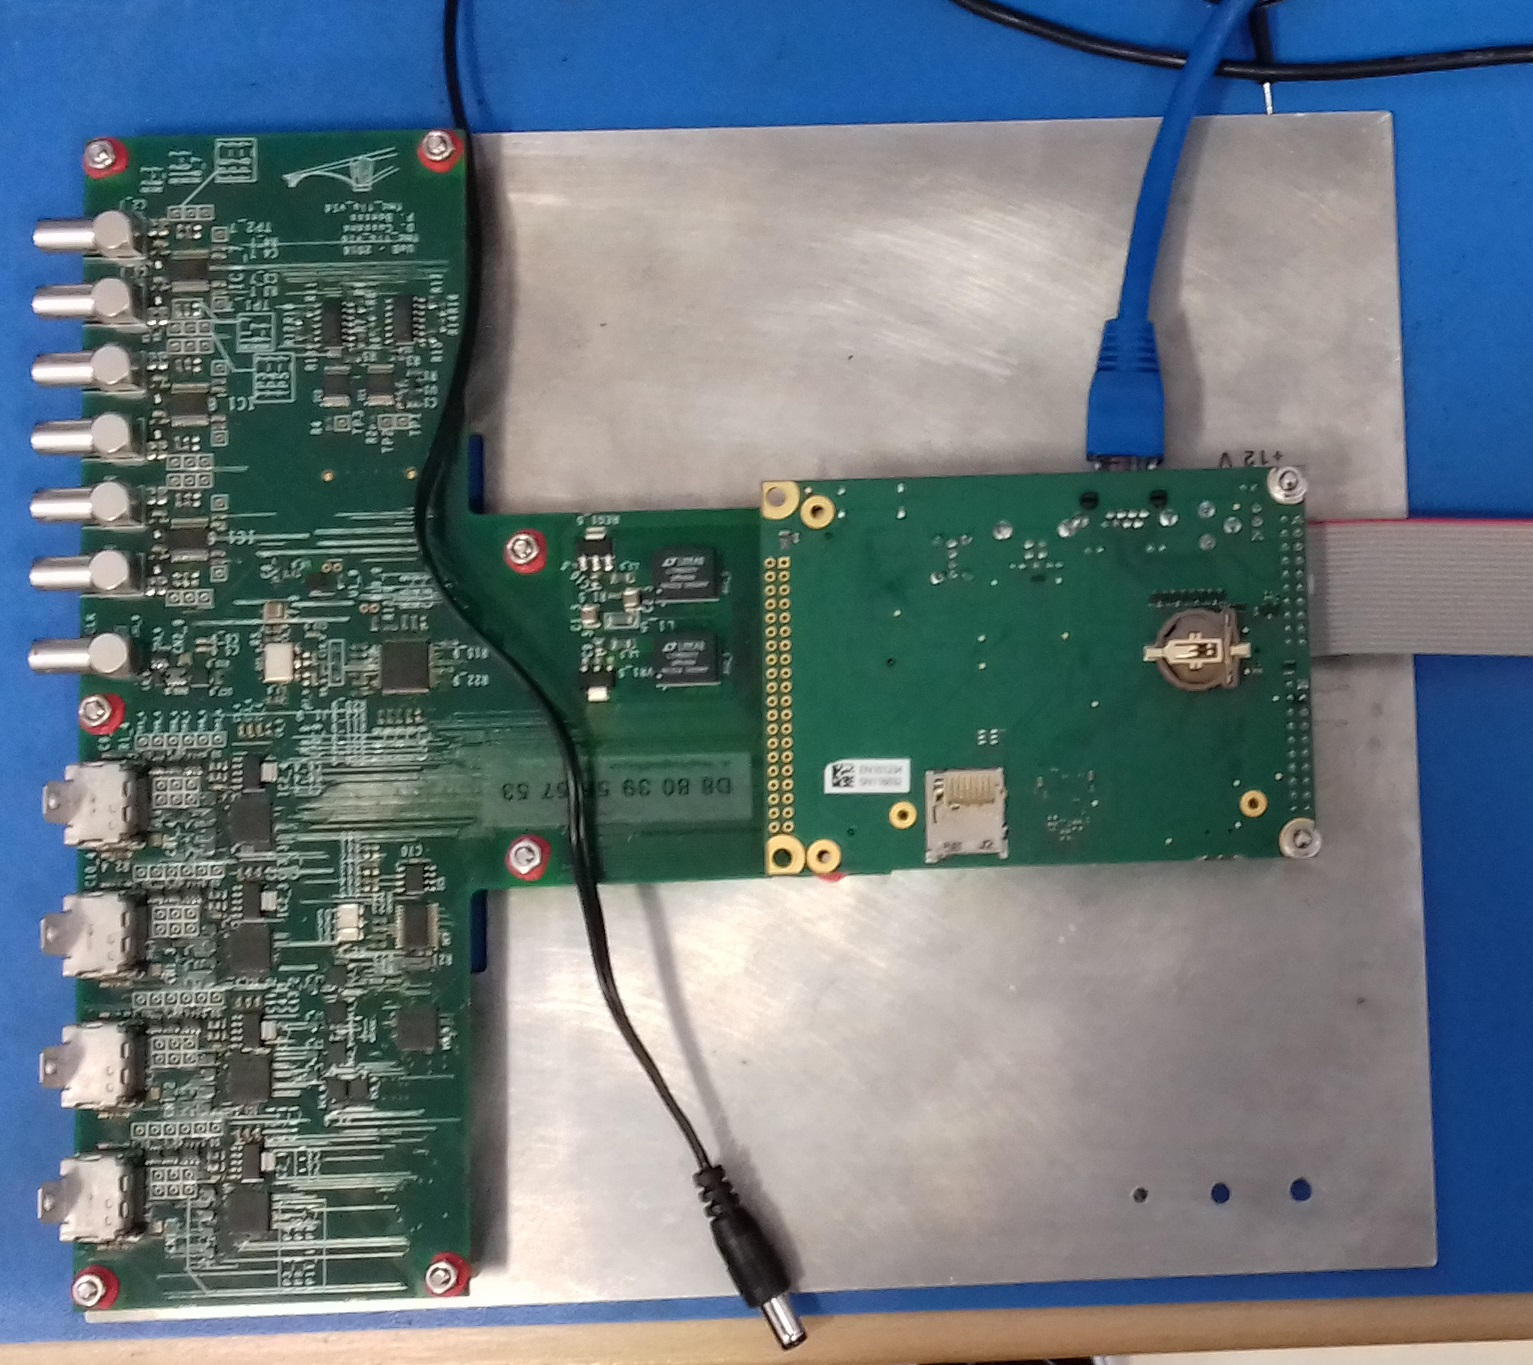
\includegraphics[width=.50\textwidth]{./Images/TLU_plate.jpg}
%  \caption{\brd and PM3 mounted on a base plate: in this configuration it is not possible to install the breakout board on the PM3 because the mountings screws are in the way.}\label{fig:TLUplate}
%\end{figure}
%\begin{figure}
%  \centering
%  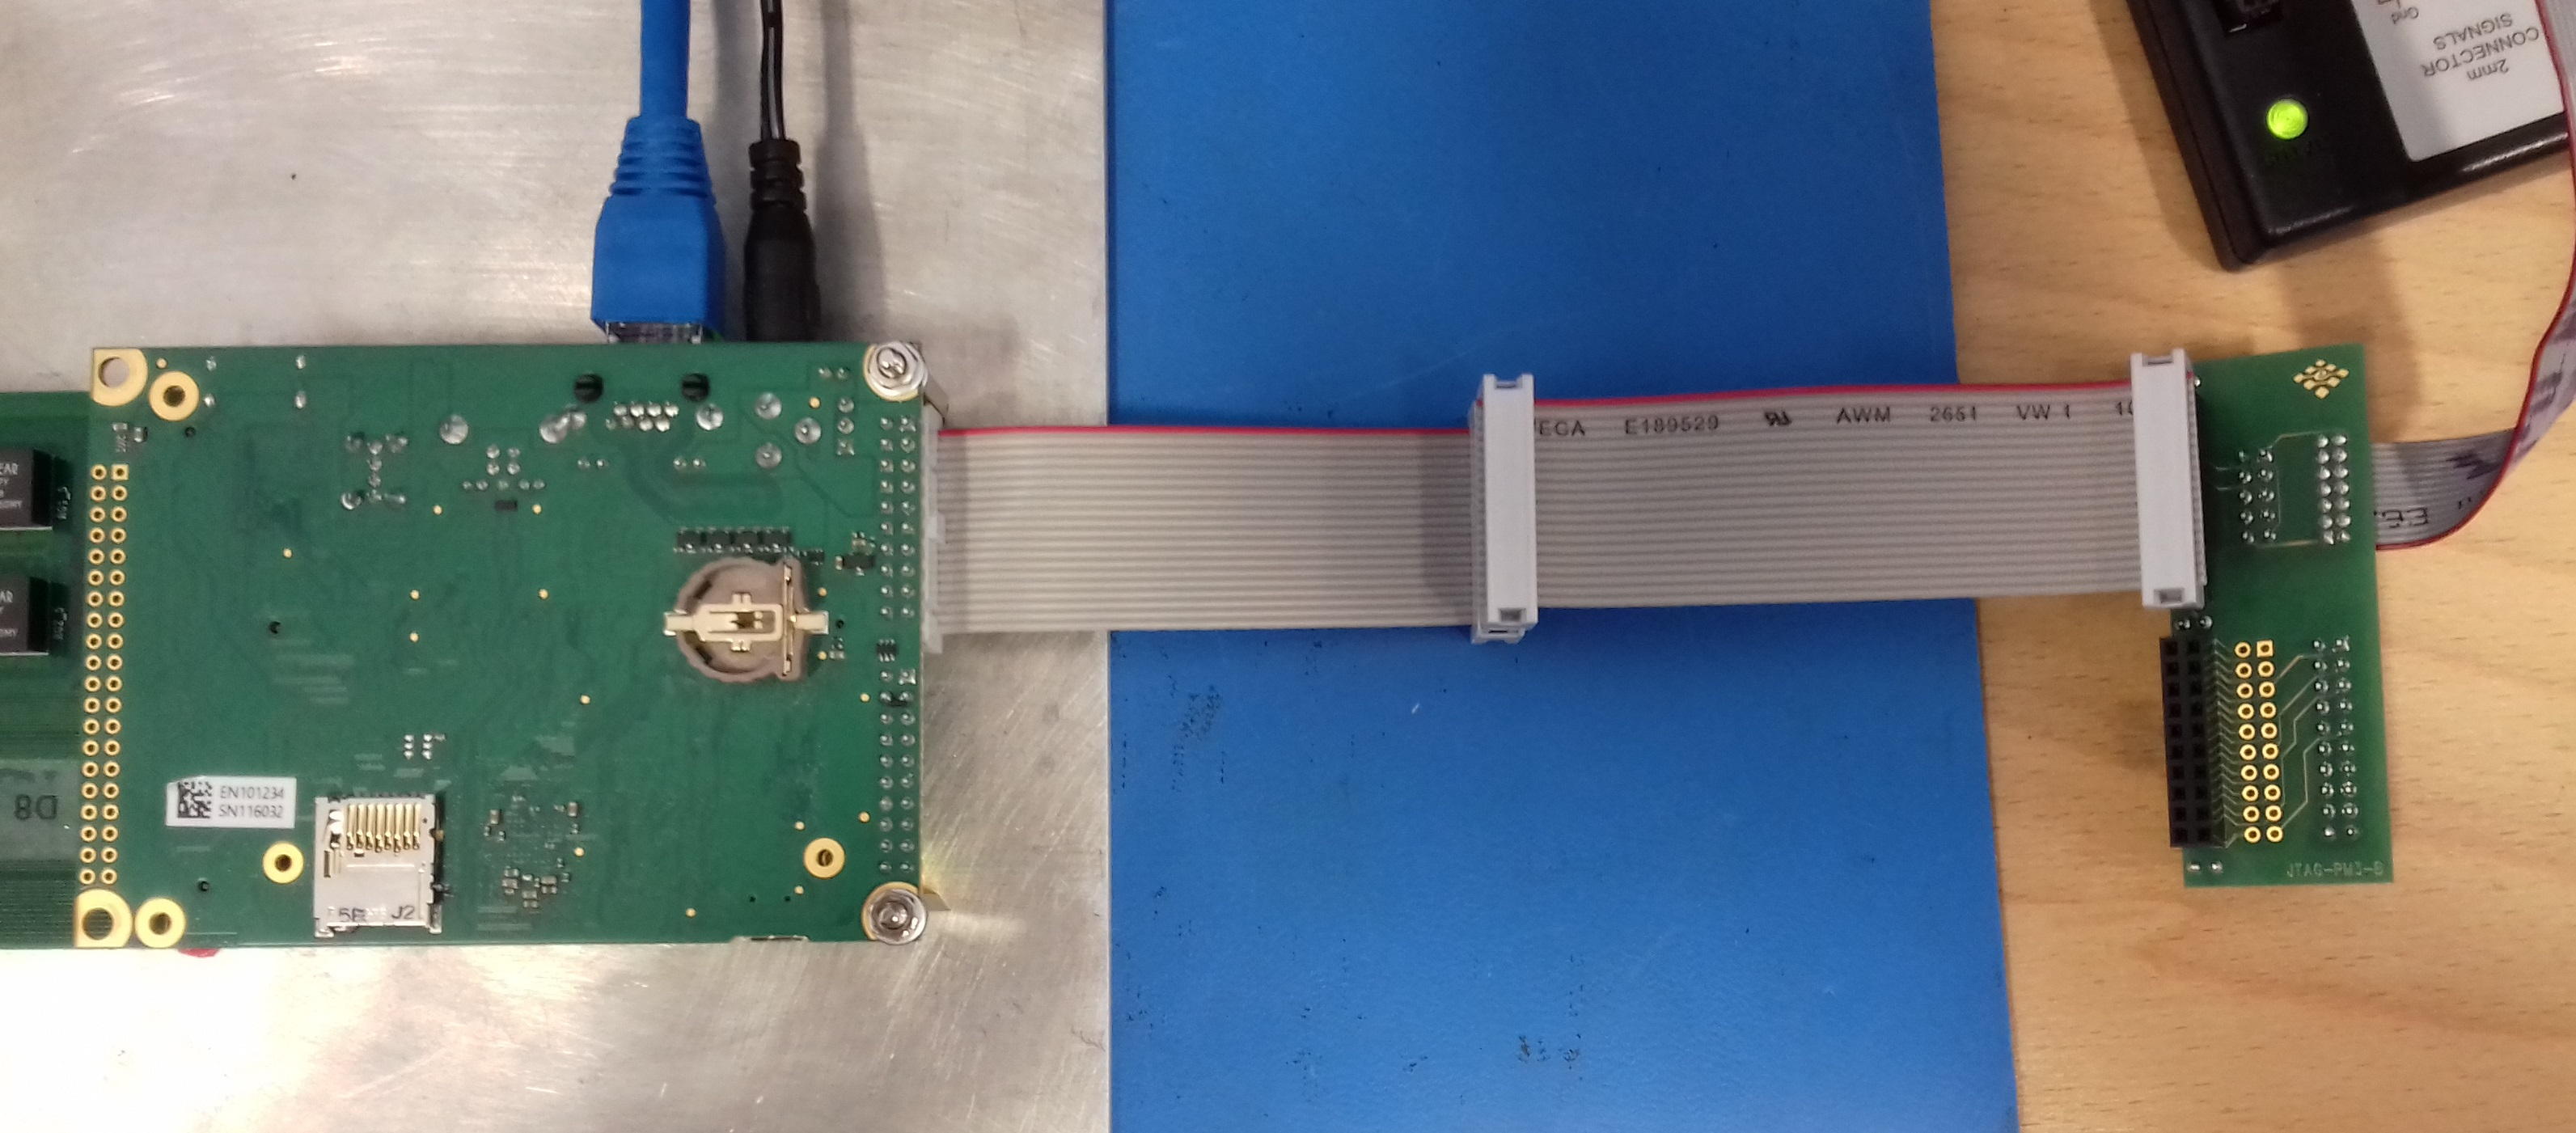
\includegraphics[width=.80\textwidth]{./Images/XilinxCable.jpg}
%  \caption{Connecting the Xilinx programming cable to the PM3 in an ugly (but effective) way.}\label{fig:XilinxCable}
%\end{figure}

\chapter{TLU Hardware}\label{ch:hardware}
Board \brd is an evolution of the miniTLU designed at the \gls{uob}. The board shares a few features with the miniTLU but also introduces several improvements. This chapter illustrates the main features of the board to provide a general view of its capabilities and an understanding of how to operate it in order to communicate with the \gls{dut}s.

\section{Inputs and interfaces}\label{ch:hwDUT}
\subsubsection{FMC}
The board must be plugged onto a \gls{fmc} carrier board with an \gls{fpga} in order to function correctly. The connection is achieved using a low pin count \gls{fmc} connector. The list of the pins used and the corresponding signal within the \gls{fpga} are provided in appendix at page~\pageref{ch:appendix}.\\

\subsubsection{Device under test}\label{ch:dut}
The \gls{dut}s are connected to the \gls{tlu} using standard size \gls{hdmi} connectors\footnote{In the miniTLU hardware there were mini\gls{hdmi} connectors.}.\\
In the current version of the hardware, up to four \gls{dut}s can be connected to the board. In this document the connectors will be referred to as \verb|HDMI1|, \verb|HDMI2|, \verb|HDMI3| and \verb|HDMI4|.\\
The connectors expect 3.3~V \gls{lvds} signals and are bi-directional, i.e. any differential pair can be configured to be an output (signal from the TLU to the DUT) or an input (signals from the DUT to the TLU) by using half-duplex line transceivers. Figure~\ref{fig:LVDSTransceiver} illustrates how the differential pairs are connected to the transceivers.
\begin{alertinfo}{Note}
    The input part of the transceiver is configured to be always on. This means that signals going \emph{into} the \gls{tlu} are always routed to the logic (\gls{fpga}). By contrast, the output transceivers have to be enabled and are off by default: signal sent from the logic to the \gls{dut}s cannot reach the devices unless the corresponding enable signal is active.
\end{alertinfo}
Table~\ref{tab:HDMIpins} shows the pin naming and the corresponding output enable signal. The clock pairs have two different enable signals to select the clock source (see section~\ref{ch:clock} for more details). In general only one of the clock sources should be active at any time.\\
The enable signals can be configured by programming two \gls{gpio} bus expanders via \gls{i2c} interface as described in section~\ref{ch:i2c}.
 \begin{table}[]
    \centering
    \caption{HDMI pin connections.}
    \label{tab:HDMIpins}
    \begin{tabular}{|l|l|l|}
    \hline
    \textbf{HDMI PIN} & \textbf{HDMI Signal Name} & \textbf{Enable Signal Name} \\ \hline
     &  &  \\ \hline
    1   & \verb|HDMI_CLK| & \begin{tabular}[c]{@{}l@{}}\verb|ENABLE_CLK_TO_DUT|\\ or\\ \verb|ENABLE_DUT_CLK_FROM_FPGA|\end{tabular} \\ \hline
    2   & \verb|GND|       & -- \\ \hline
    3   & \verb|HDMI_CLK| * & \begin{tabular}[c]{@{}l@{}}\verb|ENABLE_CLK_TO_DUT|\\ or\\ \verb|ENABLE_DUT_CLK_FROM_FPGA|\end{tabular} \\ \hline
    4   & \verb|CONT|      & \verb|ENABLE_CONT_FROM_FPGA| \\ \hline
    5   & \verb|GND|       & -- \\ \hline
    6   & \verb|CONT*|     & \verb|ENABLE_CONT_FROM_FPGA| \\ \hline
    7   & \verb|BUSY|      & \verb|ENABLE_BUSY_FROM_FPGA| \\ \hline
    8   & \verb|GND|       & -- \\ \hline
    9   & \verb|BUSY*|     & \verb|ENABLE_BUSY_FROM_FPGA| \\ \hline
    10  & \verb|SPARE|     & \verb|ENABLE_SPARE_FROM_FPGA| \\ \hline
    11  & \verb|GND|       & -- \\ \hline
    12  & \verb|SPARE*|    & \verb|ENABLE_SPARE_FROM_FPGA| \\ \hline
    13  & n.c.      &  \\ \hline
    14  & \verb|HDMI_POWER| & -- \\ \hline
    15  & \verb|TRIG|      & \verb|ENABLE_TRIG_FROM_FPGA| \\ \hline
    16  & \verb|TRIG*|     & \verb|ENABLE_TRIG_FROM_FPGA| \\ \hline
    17  & \verb|GND|       &  \\ \hline
    18  & n.c.      &  \\ \hline
    19  & n.c.      &  \\ \hline
    \end{tabular}
\end{table}
\begin{figure}
  \centering
  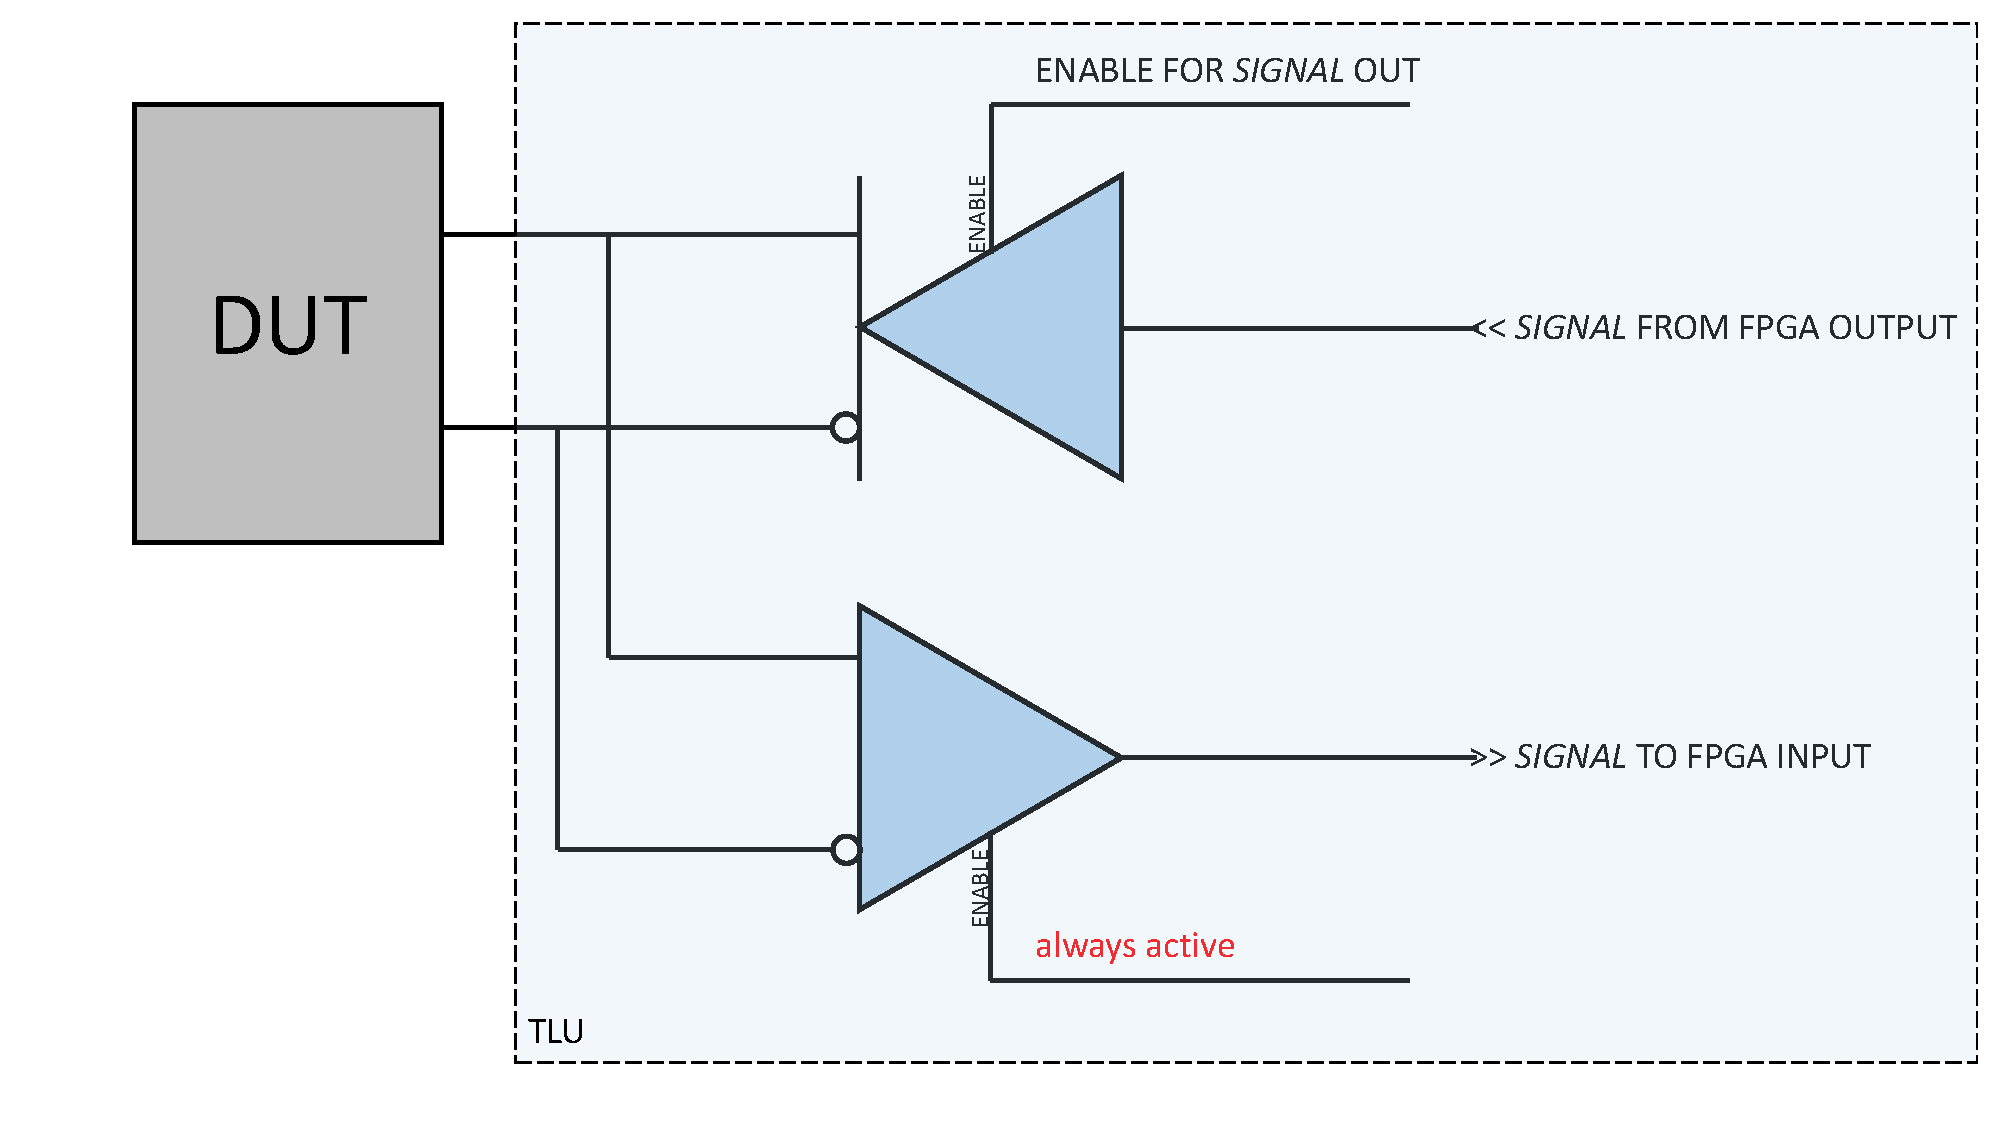
\includegraphics[width=.80\textwidth]{./Images/LVDS_transceiver.pdf}
  \caption{Internal configuration of the HDMI pins for the DUTs. The path from the DUT to the FPGA is always active. The path from the FPGA to the DUT can be enabled or disabled by the user.}\label{fig:LVDSTransceiver}
\end{figure}\\
In terms for functionalities, the four \gls{hdmi} connectors are identical with one exception: the clock signal from \verb|HDMI4| can be used as reference for the clock generator chip mounted on the hardware. For more details on this functionality refer to section~\ref{ch:clock}.

\section{Clock LEMO}
The board hosts a two-pin LEMO connector that can be used to provide a reference clock to the clock generator (see section~\ref{ch:clock}) or to output the clock from the \gls{tlu} to the external world, for instance to use it as a reference for another \gls{tlu}. The signal level is 3.3~V \gls{lvds}.\\
As for the differential pairs of the \gls{dut}s, the pins of this connector are wired to a transceiver configured to always accept the incoming signals. The outgoing direction must be enabled by using the \verb|ENABLE_CLK_TO_LEMO| signal, which can be configured using the bus expander described in in section~\ref{ch:i2c}.

\section{Trigger inputs}
Board \brd can accept up to six trigger inputs over the LEMO connectors labelled \verb|IN_1|, \verb|IN_2|, \verb|IN_3|, \verb|IN_4|, \verb|IN_5| and \verb|IN_6|. The \brd uses internal high-speed\footnote{500$\pm$30~ps propagation delay.} discriminators to detect a valid trigger signal. The voltage thresholds can be adjusted independently for each input in a range from -1.3~V to +1.3~V with 40~$\mu$V resolution.\\
The adjustment is performed by writing to two 16-bit \gls{dac}s via \gls{i2c} interface as described in section~\ref{ch:i2c}.\\
The \gls{dac}s can either use an internal reference voltage of 2.5~V or an external one of 1.3~V provided by the \gls{tlu}: it is recommended to choose the external one by configuring the appropriate register in the devices.\\
The correspondence between DAC slave and thresholds is shown in table~\ref{tab:DACOutputs}.
\begin{table}[]
\centering
\caption{DAC outputs and corresponding threshold inputs.}
\label{tab:DACOutputs}
\begin{tabular}{|l|c|c|}
\hline
                     & \multicolumn{2}{c|}{Output}                                                        \\ \hline
                     & \multicolumn{1}{l|}{\textbf{DAC2(Ic2)}} & \multicolumn{1}{l|}{\textbf{DAC1 (Ic1)}} \\ \hline
\textbf{Threshold 0} & 1                                       &                                          \\ \hline
\textbf{Threshold 1} & 0                                       &                                          \\ \hline
\textbf{Threshold 2} &                                         & 3                                        \\ \hline
\textbf{Threshold 3} &                                         & 2                                        \\ \hline
\textbf{Threshold 4} &                                         & 1                                        \\ \hline
\textbf{Threshold 5} &                                         & 0                                        \\ \hline
\end{tabular}
\end{table}


\section{I$^{2}$C slaves}\label{ch:i2c}
The \gls{i2c} interface on the \brd can be used to configured several features of the board.\\
Table~\ref{tab:I2C addresses} lists all the valid addresses and the corresponding slave on the board. The Enclustra lines refer to slaves located on the PM3 board; these slaves can be ignored with the exception of the bus expander. The Enclustra expander is used to enable/disable the \gls{i2c} lines going to the \gls{fmc} connector.
\begin{alertinfo}{Note}
    After a power cycle the Enclustra expander is configured to disable the \gls{i2c} interface pins. This means that it is impossible to communicate to any \gls{i2c} slave on the \gls{tlu} until the expander has been enabled.\\
    The interface is enable by setting bit 7 to 0 on register 0x01 of the Enclustra expander.
\end{alertinfo}
\begin{table}[]
    \centering
    \caption{I$^{2}$C addresses of the TLU. }
    \label{tab:I2C addresses}
    \begin{tabular}{|l|l|l|l|}
    \hline
    \textbf{CHIP} & \textbf{ID} & \textbf{FUNCTION}        & \textbf{ADDRESS} \\ \hline
    IC1           & AD5665RBRUZ & DAC1                     & 0x1F             \\ \hline
    IC2           & AD5665RBRUZ & DAC2                     & 0x13             \\ \hline
    IC5           & 24AA025E48T & EEPROM                   & 0x50             \\ \hline
    IC6           & PCA9539PW   & I2C Expander1            & 0x74             \\ \hline
    IC7           & PCA9539PW   & I2C Expander2            & 0x75             \\ \hline
    IC8           & ADN2814ACPZ & CDR                      & 0x60             \\ \hline
    IC8\_9        & Si5345A     & Clock Generator          & 0x68             \\ \hline
    \multicolumn{4}{|l|}{Enclustra slaves}                                                    \\ \hline
                  &             & Enclustra Bus Expander   & 0x21             \\ \hline
                  &             & Enclustra System Monitor & 0x21             \\ \hline
                  &             & Enclustra EEPROM         & 0x54             \\ \hline
                  &             & Enclustra slave          & 0x64             \\ \hline
\end{tabular}
\end{table}
Once the interface is enabled it is possible to read and write to the devices listed in the top part of table~\ref{tab:I2C addresses}.\\
The user should reference the manual of each individual component to determine the register that must be addressed. The rest of this section is meant to provide an overview of the slave functionalities.

\subsubsection{DAC}
Each \gls{dac} has four outputs that can be configured independently. \verb|DAC1| is used to configure the thresholds of the first four trigger inputs; \verb|DAC2| configures the remaining two thresholds.\\
The \gls{dac}s should be configured to use the \gls{tlu} voltage reference of 1.3~V. In these conditions, writing a value of 0x00000 to a \gls{dac} output will set the corresponding threshold to -1.3~V while a value of 0xFFFF will set it to +1.3~V.

\subsubsection{EEPROM}
The \gls{eeprom} located on the board contains a factory-set unique number, used to identify each \brd unequivocally. The number is comprised of six bytes written in as many memory locations.\\
The identifier is always in the form: \verb|0xD8 80 39 XX XX XX| with the top three bytes indicating the manufacturer and the bottom three unique to each device.

\subsubsection{Bus expander}
The expanders are used as electronic switched to enable and disable individual lines. Each expander has two 8-bit banks; the values of the bits, as well as their direction (input/output) can be configured via the \gls{i2c} interface. For the purpose of the \gls{tlu}, all the expander pins should be configured as outputs since they must drive the enable signals on the \gls{dut} transceivers.

\subsubsection{Clock and data recovery chip}
The \gls{cdr} is used in conjunction with the \gls{sfp} cage to recover data and clock from the incoming bit stream. The functionality has not yet been implemented in the firmware so the \gls{i2c} slave can be ignored for now.

\subsubsection{Clock generator}
The clock for \brd can be generated using various external or internal references (see section~\ref{ch:clock} for further details). In order to reduce any jitter from the clock source and to provide a stable clock, the board hosts a Si5345 clock generator that needs to be configured via \gls{i2c} interface.\\
The configuration involves writing $\thicksim$380 register values. A configuration file, containing all the register addresses and the corresponding values, can be generated using the ClockBuilder tool available from \href{http://www.enclustra.com/en/home/}{Silicon Labs}.\\
The registers addresses between 0x026B and 0x0272 contain user-defined values that can be used to identify the configuration version: it is advisable to check those registers and check that they contain the correct code to ensure that the chip is configured according to the \gls{tlu} specifications. As an indication, files generated for the current version of the \gls{tlu} should have a configuration identifier in the form \verb|TLU1E_XX|, where \verb|XX| is a sequential number.\\
\begin{alertinfo}{TLU Producer}
    When using the TLU producer to configure hardware, the location of the configuration file can be specified by setting the \texttt{CLOCK\_CFG\_FILE} value in the \emph{conf} file for the producer.\\
    If no value is specified, the software will look for the configuration file \texttt{../conf/confClk.txt} i.e. if the \texttt{euRun} binary file is located in \texttt{./eudaq/bin}, then the default configuration file should reside in \texttt{./eudaq/conf}. The configuration will produce an error if the file is not found.
\end{alertinfo}

\chapter{Clock}\label{ch:clock}
The \gls{tlu} can use various sources to produce a stable 40~MHz clock\footnote{For some applications a 50~MHz clock will be required instead}. A \gls{lvpecl} crystal provides the reference 50~MHz clock for a Si5345A jitter attenuator. The Si5345A can accept up to four clock sources and use them to generate the required output clocks.\\
In \brd the possible sources are: differential LEMO connector LM1\_9, one of the four \gls{hdmi} connectors (\verb|HDMI4|), a \gls{cdr} chip connected to the \gls{sfp} cage. The fourht input is used to provide a zero-delay feedback loop.\\
The low-jitter clock generated by the Si5345A can be distributed to up to ten recipients. In the \gls{tlu} these are: the four \gls{dut}s via \gls{hdmi} connectors, the differential LEMO cable, the \gls{fpga},  connector J1 as a differential pair (pins 4 and 6) and as a single ended signal (pin 8). The final output is connected to the zero-delay feedback loop.\\
The \gls{dut}s can receive the clock either from the Si5435A or directly from the \gls{fpga}: when provided by the clock generator, the signal name is \verb|CLK\_TO\_DUT| and is enabled by signal \verb|ENABLE_CLK_TO_DUT|; when the signal is provided directly from the \gls{fpga} the line used is \verb|DUT_CLK_FROM_FPGA| and is enabled by \verb|ENABLE_DUT_CLK_FROM_FPGA|.\\
The firmware uses the clock generated by the Si5345A except for the block \verb|enclustra_ax3_pm3_infra| which relies on a crystal mounted on the Enclustra board to provide the IPBus functionalities (in this way, at power up the board can communicate via IPBus even if the Si5345A is not configured).

\section{Input selection}
The Si5345 has four inputs that can be selected to provide the clock alignment; the selection can be automatic or user-defined. For further details on this aspect the user should consult the chip documentation.

\begin{table}[]
\small
\centering
\caption{Si5345  Input Selection Configuration.}
\label{tab:si5345inputs}
\begin{tabular}{|l|l|l|}
\hline
\textbf{Register Name} & \textbf{Hex Address {[}Bit Field{]}} & \textbf{Function}                                                                                                                                                                                                                              \\ \hline
CLK\_SWITCH\_MODE      & 0x0536{[}1:0{]}                      & \begin{tabular}[c]{@{}l@{}}Selects manual or automatic switching modes.\\ Automatic mode can be revertive or non-revertive.\\ Selections are the following:\\00 Manual\\01 Automatic non-revertive\\02 Automatic revertive\\03 Reserved\end{tabular} \\ \hline
IN\_SEL\_REGCTRL       & 0x052A {[}0{]}                       & \begin{tabular}[c]{@{}l@{}}0 for pin controlled clock selection\\ 1 for register controlled clock selection\end{tabular}                                                                                                                       \\ \hline
IN\_SEL                & 0x052A {[}2:1{]}                     & \begin{tabular}[c]{@{}l@{}}0 for IN0\\ 1 for IN1\\ 2 for IN2\\ 3 for IN3 (or FB\_IN)\end{tabular}                                                                                                                                              \\ \hline
\end{tabular}
\end{table}


\section{Logic clocks registers}\label{ch:logicClock}
LogicClocksCSR: in the new TLU the selection of the clock source is done by programming the Si5345. As a consequence, there is no reason to write to this register. Reading it back returns the status of the PLL on bit 0, so this should read 0x1. 
\chapter{DUT signals}\label{ch:DUTsignals}
In the old versions of the \gls{tlu} the direction of the signals on the \verb|HDMI*| connectors were pre-defined. The new hardware has separate lines for signals going into the \gls{tlu} and signals out of the \gls{tlu}. See section~\ref{ch:hwDUT} for further details.\\ 
\chapter{Trigger inputs}\label{ch:triggerinputs}
The six inputs on the \gls{tlu} can be used to generate a global trigger that is then issued to all the \gls{dut}s.\\
Each input has a programmable voltage discriminator that can be configured in the range [-1.3 : 1.3]~V.\\
All the inputs are protected by clamping diodes that limit the input voltage in the range [-5 : +5]~V.

\section{Trigger logic}\label{ch:triggerLogic}
The TLU has six trigger inputs than can be used to generate a valid trigger event. The number of possible different trigger combinations is $2^6= 64$ so a 64-bit word can be used to decide the valid combinations. In the hardware the 64-bit word is split into two 32-bit words (indicated as \gls{msb} and \gls{lsb} word) and the rules to generate the trigger can be specified by the user by writing in the two 32-bit registers \verb|TriggerPattern_highW| and \verb|TriggerPattern_lowW|: the first stores the 32 most significative bits of the trigger word, the latter stores the least significative bits.\\
The user can select any combination of the trigger inputs and declare it a valid trigger pattern by setting a 1 in the corresponding trigger configuration word.
Tables~\ref{tab:trigconfigLow} and ~\ref{tab:trigconfigHigh} show an example of how to determine the trigger configuration words: whenever a valid trigger combination is encountered, the user should put a 1 in the corresponding row under the PATTERN column. The pattern thus obtained is the required word to write in the configuration register.\\
It is important to note that this solution allows the user to set veto pattern as well: for instance if only word 31 from table~\ref{tab:trigconfigLow} were picked, then the \gls{tlu} would only register a trigger when the combination $\overline{I_{5}}$ * $I_{4}$ * $I_{3}$ * $I_{2}$ * $I_{1}$ * $I_{0}$ was presented at its inputs. In other words, in this specific case $I_{5}$ would act as a veto signal and the \gls{tlu} would \textbf{not} produce a trigger if $I_{5}$=1.

% Please add the following required packages to your document preamble:
% \usepackage{multirow}
\begin{table}[]
\centering
\caption{Example of configuration word for the least significative bits of the trigger registers: the only valid configuration is represented by $\overline{I_{5}}$ + $I_{4}$ + $I_{3}$ + $I_{2}$ + $I_{1}$ + $I_{0}$, i.e. a trigger is accepted if all the inputs, except $I_{5}$, present a logic 1 at the same time. The user would then write the resulting word 0x80000000 in the TriggerPattern\_lowW register.}
\label{tab:trigconfigLow}
\begin{tabular}{|l|l|l|l|l|l|l||c||c|l|r|}
\hline
DEC & I5 & I4 & I3 & I2 & I1 & I0 & PATTERN & \multicolumn{1}{l|}{\begin{tabular}[c]{@{}l@{}}CONFIG. \\ WORD\end{tabular}} &                                  & $2^{n}$ \\ \hline
0  & 0  & 0  & 0  & 0  & 0  & 0  & \rotatebox[origin=c]{90}{0}       & \parbox[t]{2mm}{\multirow{4}{*}{\rotatebox[origin=c]{90}{0}}}                                                                & \parbox[t]{2mm}{\multirow{32}{*}{\rotatebox[origin=c]{90}{LOWEST 32-bits}}} & 1                   \\ \cline{1-8} \cline{11-11}
1  & 0  & 0  & 0  & 0  & 0  & 1  & \rotatebox[origin=c]{90}{0}       &                                                                                    &                                  & 2                   \\ \cline{1-8} \cline{11-11}
2  & 0  & 0  & 0  & 0  & 1  & 0  & \rotatebox[origin=c]{90}{0}       &                                                                                    &                                  & 4                   \\ \cline{1-8} \cline{11-11}
3  & 0  & 0  & 0  & 0  & 1  & 1  & \rotatebox[origin=c]{90}{0}       &                                                                                    &                                  & 8                   \\ \cline{1-9} \cline{11-11}
4  & 0  & 0  & 0  & 1  & 0  & 0  & \rotatebox[origin=c]{90}{0}       & \parbox[t]{2mm}{\multirow{4}{*}{\rotatebox[origin=c]{90}{0}}}                                                                  &                                  & 16                  \\ \cline{1-8} \cline{11-11}
5  & 0  & 0  & 0  & 1  & 0  & 1  & \rotatebox[origin=c]{90}{0}       &                                                                                    &                                  & 32                  \\ \cline{1-8} \cline{11-11}
6  & 0  & 0  & 0  & 1  & 1  & 0  & \rotatebox[origin=c]{90}{0}       &                                                                                    &                                  & 64                  \\ \cline{1-8} \cline{11-11}
7  & 0  & 0  & 0  & 1  & 1  & 1  & \rotatebox[origin=c]{90}{0}       &                                                                                    &                                  & 128                 \\ \cline{1-9} \cline{11-11}
8  & 0  & 0  & 1  & 0  & 0  & 0  & \rotatebox[origin=c]{90}{0}       & \parbox[t]{2mm}{\multirow{4}{*}{\rotatebox[origin=c]{90}{0}}}                                                                  &                                  & 256                 \\ \cline{1-8} \cline{11-11}
9  & 0  & 0  & 1  & 0  & 0  & 1  & \rotatebox[origin=c]{90}{0}       &                                                                                    &                                  & 512                 \\ \cline{1-8} \cline{11-11}
10  & 0  & 0  & 1  & 0  & 1  & 0  & \rotatebox[origin=c]{90}{0}       &                                                                                    &                                  & 1024                \\ \cline{1-8} \cline{11-11}
11  & 0  & 0  & 1  & 0  & 1  & 1  & \rotatebox[origin=c]{90}{0}       &                                                                                    &                                  & 2048                \\ \cline{1-9} \cline{11-11}
12  & 0  & 0  & 1  & 1  & 0  & 0  & \rotatebox[origin=c]{90}{0}       & \parbox[t]{2mm}{\multirow{4}{*}{\rotatebox[origin=c]{90}{0}}}                                                                 &                                  & 4096                \\ \cline{1-8} \cline{11-11}
13  & 0  & 0  & 1  & 1  & 0  & 1  & \rotatebox[origin=c]{90}{0}       &                                                                                    &                                  & 8192                \\ \cline{1-8} \cline{11-11}
14  & 0  & 0  & 1  & 1  & 1  & 0  & \rotatebox[origin=c]{90}{0}       &                                                                                    &                                  & 16384               \\ \cline{1-8} \cline{11-11}
15  & 0  & 0  & 1  & 1  & 1  & 1  & \rotatebox[origin=c]{90}{0}       &                                                                                    &                                  & 32768               \\ \cline{1-9} \cline{11-11}
16  & 0  & 1  & 0  & 0  & 0  & 0  & \rotatebox[origin=c]{90}{0}       & \parbox[t]{2mm}{\multirow{4}{*}{\rotatebox[origin=c]{90}{0}}}                                                                 &                                  & 65536               \\ \cline{1-8} \cline{11-11}
17  & 0  & 1  & 0  & 0  & 0  & 1  & \rotatebox[origin=c]{90}{0}       &                                                                                    &                                  & 131072              \\ \cline{1-8} \cline{11-11}
18  & 0  & 1  & 0  & 0  & 1  & 0  & \rotatebox[origin=c]{90}{0}       &                                                                                    &                                  & 262144              \\ \cline{1-8} \cline{11-11}
19  & 0  & 1  & 0  & 0  & 1  & 1  & \rotatebox[origin=c]{90}{0}       &                                                                                    &                                  & 524288              \\ \cline{1-9} \cline{11-11}
20  & 0  & 1  & 0  & 1  & 0  & 0  & \rotatebox[origin=c]{90}{0}       & \parbox[t]{2mm}{\multirow{4}{*}{\rotatebox[origin=c]{90}{0}}}                                                                 &                                  & 1048576             \\ \cline{1-8} \cline{11-11}
21  & 0  & 1  & 0  & 1  & 0  & 1  & \rotatebox[origin=c]{90}{0}       &                                                                                    &                                  & 2097152             \\ \cline{1-8} \cline{11-11}
22  & 0  & 1  & 0  & 1  & 1  & 0  & \rotatebox[origin=c]{90}{0}       &                                                                                    &                                  & 4194304             \\ \cline{1-8} \cline{11-11}
23  & 0  & 1  & 0  & 1  & 1  & 1  & \rotatebox[origin=c]{90}{0}       &                                                                                    &                                  & 8388608             \\ \cline{1-9} \cline{11-11}
24  & 0  & 1  & 1  & 0  & 0  & 0  & \rotatebox[origin=c]{90}{0}       & \parbox[t]{2mm}{\multirow{4}{*}{\rotatebox[origin=c]{90}{0}}}                                                                 &                                  & 16777216            \\ \cline{1-8} \cline{11-11}
25  & 0  & 1  & 1  & 0  & 0  & 1  & \rotatebox[origin=c]{90}{0}       &                                                                                    &                                  & 33554432            \\ \cline{1-8} \cline{11-11}
26  & 0  & 1  & 1  & 0  & 1  & 0  & \rotatebox[origin=c]{90}{0}       &                                                                                    &                                  & 67108864            \\ \cline{1-8} \cline{11-11}
27  & 0  & 1  & 1  & 0  & 1  & 1  & \rotatebox[origin=c]{90}{0}       &                                                                                    &                                  & 134217728           \\ \cline{1-9} \cline{11-11}
28  & 0  & 1  & 1  & 1  & 0  & 0  & \rotatebox[origin=c]{90}{0}       & \parbox[t]{2mm}{\multirow{4}{*}{\rotatebox[origin=c]{90}{8}}}                                                                 &                                  & 268435456           \\ \cline{1-8} \cline{11-11}
29  & 0  & 1  & 1  & 1  & 0  & 1  & \rotatebox[origin=c]{90}{0}       &                                                                                    &                                  & 536870912           \\ \cline{1-8} \cline{11-11}
30  & 0  & 1  & 1  & 1  & 1  & 0  & \rotatebox[origin=c]{90}{0}       &                                                                                    &                                  & 1073741824          \\ \cline{1-8} \cline{11-11}
31  & 0  & 1  & 1  & 1  & 1  & 1  & \rotatebox[origin=c]{90}{1}       &                                                                                    &                                  & 2147483648          \\ \hline
\end{tabular}
\end{table}



\begin{table}[]
\centering
\caption{Example of the most significative word of the register: a valid trigger is obtained when the inputs show the same configuration as row DEC 36, 37, 38, 39, 41, 43 and 63. These configuration are in logic OR with that presented in table~\ref{tab:trigconfigLow}. The resulting configuration word is 0x80000AF0.}
\label{tab:trigconfigHigh}
\begin{tabular}{|l|l|l|l|l|l|l||c||c|l|r|}
\hline
DEC & I5 & I4 & I3 & I2 & I1 & I0 & PATTERN & \multicolumn{1}{l|}{\begin{tabular}[c]{@{}l@{}}CONFIG. \\ WORD\end{tabular}} &                                  & $2^{n}$ \\ \hline
32  & 1  & 0  & 0  & 0  & 0  & 0  & \rotatebox[origin=c]{90}{0}       & \parbox[t]{2mm}{\multirow{4}{*}{\rotatebox[origin=c]{90}{0}}}                                                                & \parbox[t]{2mm}{\multirow{32}{*}{\rotatebox[origin=c]{90}{HIGHEST 32-bits}}} & 1                   \\ \cline{1-8} \cline{11-11}
33  & 1  & 0  & 0  & 0  & 0  & 1  & \rotatebox[origin=c]{90}{0}       &                                                                                    &                                  & 2                   \\ \cline{1-8} \cline{11-11}
34  & 1  & 0  & 0  & 0  & 1  & 0  & \rotatebox[origin=c]{90}{0}       &                                                                                    &                                  & 4                   \\ \cline{1-8} \cline{11-11}
35  & 1  & 0  & 0  & 0  & 1  & 1  & \rotatebox[origin=c]{90}{0}       &                                                                                    &                                  & 8                   \\ \cline{1-9} \cline{11-11}
36  & 1  & 0  & 0  & 1  & 0  & 0  & \rotatebox[origin=c]{90}{1}       & \parbox[t]{2mm}{\multirow{4}{*}{\rotatebox[origin=c]{90}{F}}}                                                                  &                                  & 16                  \\ \cline{1-8} \cline{11-11}
37  & 1  & 0  & 0  & 1  & 0  & 1  & \rotatebox[origin=c]{90}{1}       &                                                                                    &                                  & 32                  \\ \cline{1-8} \cline{11-11}
38  & 1  & 0  & 0  & 1  & 1  & 0  & \rotatebox[origin=c]{90}{1}       &                                                                                    &                                  & 64                  \\ \cline{1-8} \cline{11-11}
39  & 1  & 0  & 0  & 1  & 1  & 1  & \rotatebox[origin=c]{90}{1}       &                                                                                    &                                  & 128                 \\ \cline{1-9} \cline{11-11}
40  & 1  & 0  & 1  & 0  & 0  & 0  & \rotatebox[origin=c]{90}{0}       & \parbox[t]{2mm}{\multirow{4}{*}{\rotatebox[origin=c]{90}{A}}}                                                                  &                                  & 256                 \\ \cline{1-8} \cline{11-11}
41  & 1  & 0  & 1  & 0  & 0  & 1  & \rotatebox[origin=c]{90}{1}       &                                                                                    &                                  & 512                 \\ \cline{1-8} \cline{11-11}
42  & 1  & 0  & 1  & 0  & 1  & 0  & \rotatebox[origin=c]{90}{0}       &                                                                                    &                                  & 1024                \\ \cline{1-8} \cline{11-11}
43  & 1  & 0  & 1  & 0  & 1  & 1  & \rotatebox[origin=c]{90}{1}       &                                                                                    &                                  & 2048                \\ \cline{1-9} \cline{11-11}
44  & 1  & 0  & 1  & 1  & 0  & 0  & \rotatebox[origin=c]{90}{0}       & \parbox[t]{2mm}{\multirow{4}{*}{\rotatebox[origin=c]{90}{0}}}                                                                 &                                  & 4096                \\ \cline{1-8} \cline{11-11}
45  & 1  & 0  & 1  & 1  & 0  & 1  & \rotatebox[origin=c]{90}{0}       &                                                                                    &                                  & 8192                \\ \cline{1-8} \cline{11-11}
46  & 1  & 0  & 1  & 1  & 1  & 0  & \rotatebox[origin=c]{90}{0}       &                                                                                    &                                  & 16384               \\ \cline{1-8} \cline{11-11}
47  & 1  & 0  & 1  & 1  & 1  & 1  & \rotatebox[origin=c]{90}{0}       &                                                                                    &                                  & 32768               \\ \cline{1-9} \cline{11-11}
48  & 1  & 1  & 0  & 0  & 0  & 0  & \rotatebox[origin=c]{90}{0}       & \parbox[t]{2mm}{\multirow{4}{*}{\rotatebox[origin=c]{90}{0}}}                                                                 &                                  & 65536               \\ \cline{1-8} \cline{11-11}
49  & 1  & 1  & 0  & 0  & 0  & 1  & \rotatebox[origin=c]{90}{0}       &                                                                                    &                                  & 131072              \\ \cline{1-8} \cline{11-11}
50  & 1  & 1  & 0  & 0  & 1  & 0  & \rotatebox[origin=c]{90}{0}       &                                                                                    &                                  & 262144              \\ \cline{1-8} \cline{11-11}
51  & 1  & 1  & 0  & 0  & 1  & 1  & \rotatebox[origin=c]{90}{0}       &                                                                                    &                                  & 524288              \\ \cline{1-9} \cline{11-11}
52  & 1  & 1  & 0  & 1  & 0  & 0  & \rotatebox[origin=c]{90}{0}       & \parbox[t]{2mm}{\multirow{4}{*}{\rotatebox[origin=c]{90}{0}}}                                                                 &                                  & 1048576             \\ \cline{1-8} \cline{11-11}
53  & 1  & 1  & 0  & 1  & 0  & 1  & \rotatebox[origin=c]{90}{0}       &                                                                                    &                                  & 2097152             \\ \cline{1-8} \cline{11-11}
54  & 1  & 1  & 0  & 1  & 1  & 0  & \rotatebox[origin=c]{90}{0}       &                                                                                    &                                  & 4194304             \\ \cline{1-8} \cline{11-11}
55  & 1  & 1  & 0  & 1  & 1  & 1  & \rotatebox[origin=c]{90}{0}       &                                                                                    &                                  & 8388608             \\ \cline{1-9} \cline{11-11}
56  & 1  & 1  & 1  & 0  & 0  & 0  & \rotatebox[origin=c]{90}{0}       & \parbox[t]{2mm}{\multirow{4}{*}{\rotatebox[origin=c]{90}{0}}}                                                                 &                                  & 16777216            \\ \cline{1-8} \cline{11-11}
57  & 1  & 1  & 1  & 0  & 0  & 1  & \rotatebox[origin=c]{90}{0}       &                                                                                    &                                  & 33554432            \\ \cline{1-8} \cline{11-11}
58  & 1  & 1  & 1  & 0  & 1  & 0  & \rotatebox[origin=c]{90}{0}       &                                                                                    &                                  & 67108864            \\ \cline{1-8} \cline{11-11}
59  & 1  & 1  & 1  & 0  & 1  & 1  & \rotatebox[origin=c]{90}{0}       &                                                                                    &                                  & 134217728           \\ \cline{1-9} \cline{11-11}
60  & 1  & 1  & 1  & 1  & 0  & 0  & \rotatebox[origin=c]{90}{0}       & \parbox[t]{2mm}{\multirow{4}{*}{\rotatebox[origin=c]{90}{8}}}                                                                 &                                  & 268435456           \\ \cline{1-8} \cline{11-11}
61  & 1  & 1  & 1  & 1  & 0  & 1  & \rotatebox[origin=c]{90}{0}       &                                                                                    &                                  & 536870912           \\ \cline{1-8} \cline{11-11}
62  & 1  & 1  & 1  & 1  & 1  & 0  & \rotatebox[origin=c]{90}{0}       &                                                                                    &                                  & 1073741824          \\ \cline{1-8} \cline{11-11}
63  & 1  & 1  & 1  & 1  & 1  & 1  & \rotatebox[origin=c]{90}{1}       &                                                                                    &                                  & 2147483648          \\ \hline
\end{tabular}
\end{table}
\noindent The default configuration in the firmware is Hi=~0xFFFFFFFF, Low=~0xFFFEFFFE, which means that as long as any trigger input fires, a trigger will be generated. These words are loaded in the \gls{fpga} every time the firmware is flushed.\\

\begin{alertinfo}{Trigger logic definition}
    The user should pay attention to what trigger logic they want to define in order to avoid confusion in the data.\\
    A ``1'' in the logic table means that the corresponding input must be active to produce a valid trigger. Similarly, a ``0'' indicates that the corresponding input must be inactive (i.e. is a veto, not an ignore). Any change in input configuration will cause the logic to re-assess the trigger status. The following section gives a brief example.\\
\end{alertinfo}

\begin{alertinfo}{Bit 0 meaning}
    A 1 in the lowest bit of the \gls{lsb} word indicates that $\overline{I_{5}}$ * $\overline{I_{4}}$ * $\overline{I_{3}}$ * $\overline{I_{2}}$ * $\overline{I_{1}}$ * $\overline{I_{0}}$ is a valid trigger combination, so the \gls{tlu} will produce a trigger when all the inputs are unactive (i.e. even if all the inputs are unplugged). Apart from very specific cases, this is generally not a desired behaviour.
\end{alertinfo}

\subsubsection{Example}
In this example we have connected a pulser to two inputs of the \gls{tlu}, namely \verb|IN_1| and \verb|IN_5|. The inputs fire with a small, random delay with respect to each other.\\
In order to ensure that the signals overlap adequately, we use the \emph{stretch} register (see chapter~\ref{ch:triggerLogic}) to increase the length of the pulses: we extend \emph{in0} to 10 clock cycles and \emph{in4} to 8 clock cycles, where the clock has a frequency of 160~MHz. The resulting signals are shown in figure~\ref{Fig:exampleExtendedTriggers}.
\begin{figure}
  \centering
  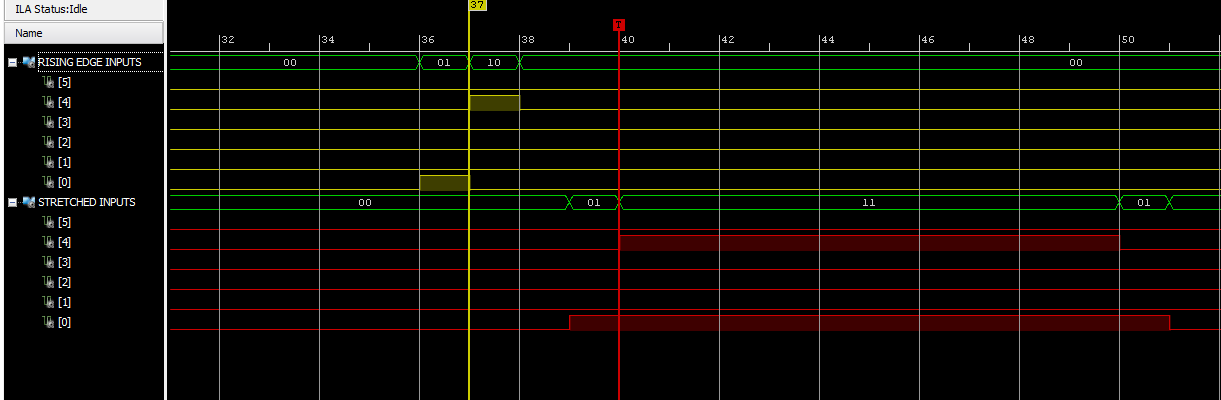
\includegraphics[width=.90\textwidth]{./Images/Initial.png}
  \caption{Input pulses (yellow) and corresponding stretched signals (red). Input 0 is stretched by 10 cycles, input 4 by 8, hence the difference in pulse widths.}
  \label{Fig:exampleExtendedTriggers}
\end{figure}\\
We can now define the trigger logic to be used to assert a valid trigger: we only consider the lower 32-bits of the trigger word and see how different values can produce very different results.
\begin{itemize}
    \item Trigger \gls{lsb} word= 0x00020000. This indicates that the only valid trigger combination occurs when both \verb|IN_1| and \verb|IN_5| are high. The valid trigger goes high 1 clock cycle after this condition is met and remains high up to 1 clock cycle after the condition is no longer valid. This is illustrated in figure~\ref{Fig:exampleTrig00020000}.
        \begin{figure}
            \centering
            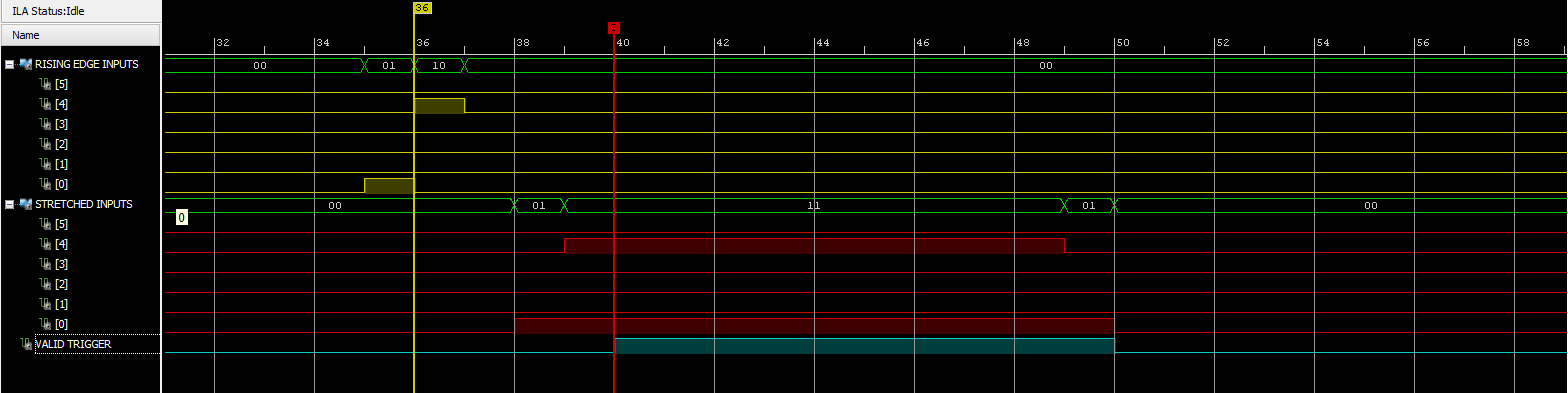
\includegraphics[width=.90\textwidth]{./Images/Trigger0x00020000.png}
            \caption{Trigger configuration 0x00020000. The valid trigger (blue) is asserted only when both signals are high. This condition occurs at frame 39. The trigger is asserted on the following frame.}
            \label{Fig:exampleTrig00020000}
        \end{figure}\\
    \item Trigger \gls{lsb} word= 0x00020002. This indicates that a valid trigger is achieved in two separated configurations (in logic OR): when both inputs are high at the same time (as in the previous case) or if \verb|IN_1| is active on its own. This is illustrated in figure~\ref{Fig:exampleTrig00020002}. It can be seen that the valid trigger is asserted immediately one clock cycle after \verb|IN_1| is high and remains high as long as this condition is met. One might assume that specifying the combination with \verb|IN_5| is redundant, but the following example should show that this is not the case.
        \begin{figure}
            \centering
            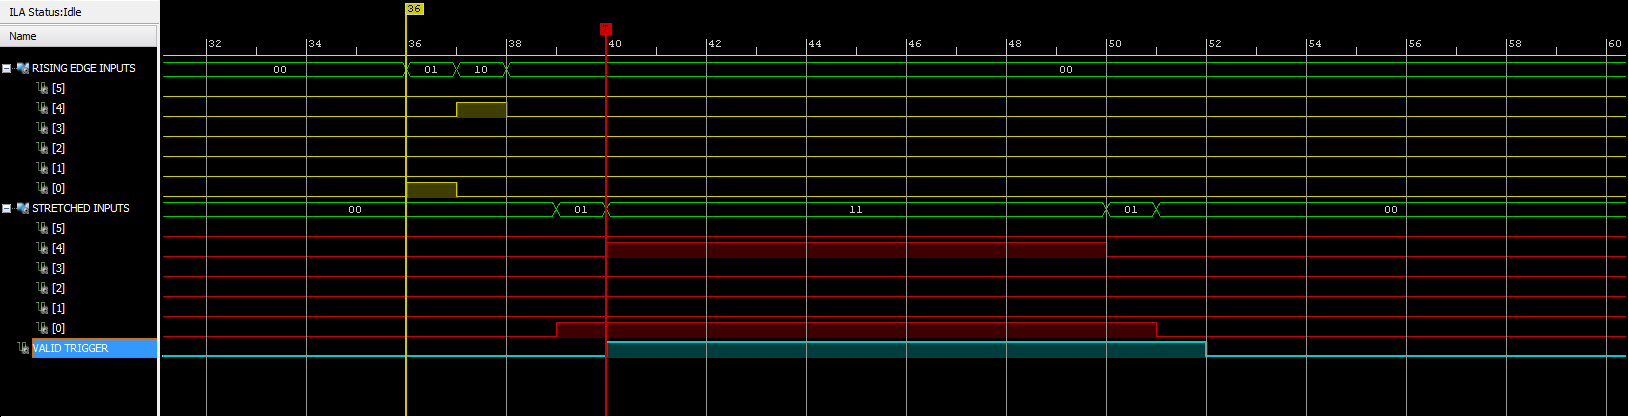
\includegraphics[width=.90\textwidth]{./Images/Trigger0x00020002.png}
            \caption{Trigger configuration 0x00020002. The valid trigger (blue) is asserted if \texttt{IN\_1} is high OR when \texttt{IN\_1} and \texttt{IN\_5} are both high at the same time.}
            \label{Fig:exampleTrig00020002}
        \end{figure}\\
    \item Trigger \gls{lsb} word= 0x00000002. This indicates that the only valid configuration is the one where only \verb|IN_1| is high. It is important to understand that in this configuration all other inputs act as veto. This might produce unexpected results if the user is not careful\footnote{Specifically, pulse stretch, pulse delay and trigger logic must be configured correctly to avoid unwanted results.}.\\
        In figure~\ref{Fig:exampleTrig00000002} it is possible to see that the logic produces two separated trigger valid pulses, both shorter than the ones in previous examples: the first one is due to \verb|IN_1| going high while \verb|IN_5| is low. As soon as \verb|IN_5| goes high, the trigger condition is no longer met. When \verb|IN_5| returns low, a trigger condition is met again because \verb|IN_1| is still high. In this specific case, the double pulse is caused by the different width of the pulses.
        \begin{figure}
            \centering
            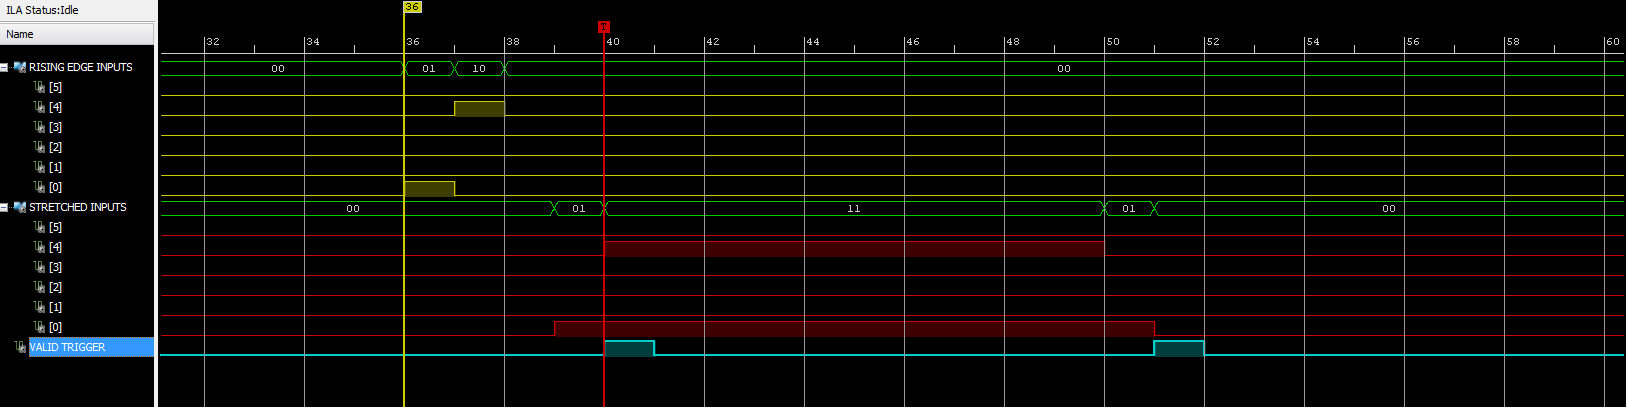
\includegraphics[width=.90\textwidth]{./Images/Trigger0x00000002.png}
            \caption{Trigger configuration 0x00000002. The valid trigger (blue) is asserted only when \texttt{IN\_1} is active on its own. As such, two separated trigger pulses are produced because \texttt{IN\_5} goes high and returns low before \texttt{IN\_1}.}
            \label{Fig:exampleTrig00000002}
        \end{figure}\\
\end{itemize}

\section{Stretch and delay}
The trigger logic is designed to detect edge transitions\footnote{Currently only negative edges are registered.} at the trigger inputs and produce a pulse for each transition detected. The pulse has an initial duration of one clock cycle (f= 160~MHz, one cycle 6.25~ns) and occurs on the next rising edge of the 160~MHz internal clock.\\
Each pulse can be stretched and delayed in integer numbers of clock cycles to compensate for differences in cable length. Two separate 5-bit registers are used for the task: the value written in the registers will stretch/delay the pulse by a corresponding number of clock cycles.\\
Diagram~\ref{Fig:trigger_stretchdelay} shows the effect of the delay and stretch words on the trigger logic.
\begin{figure}
  \centering
  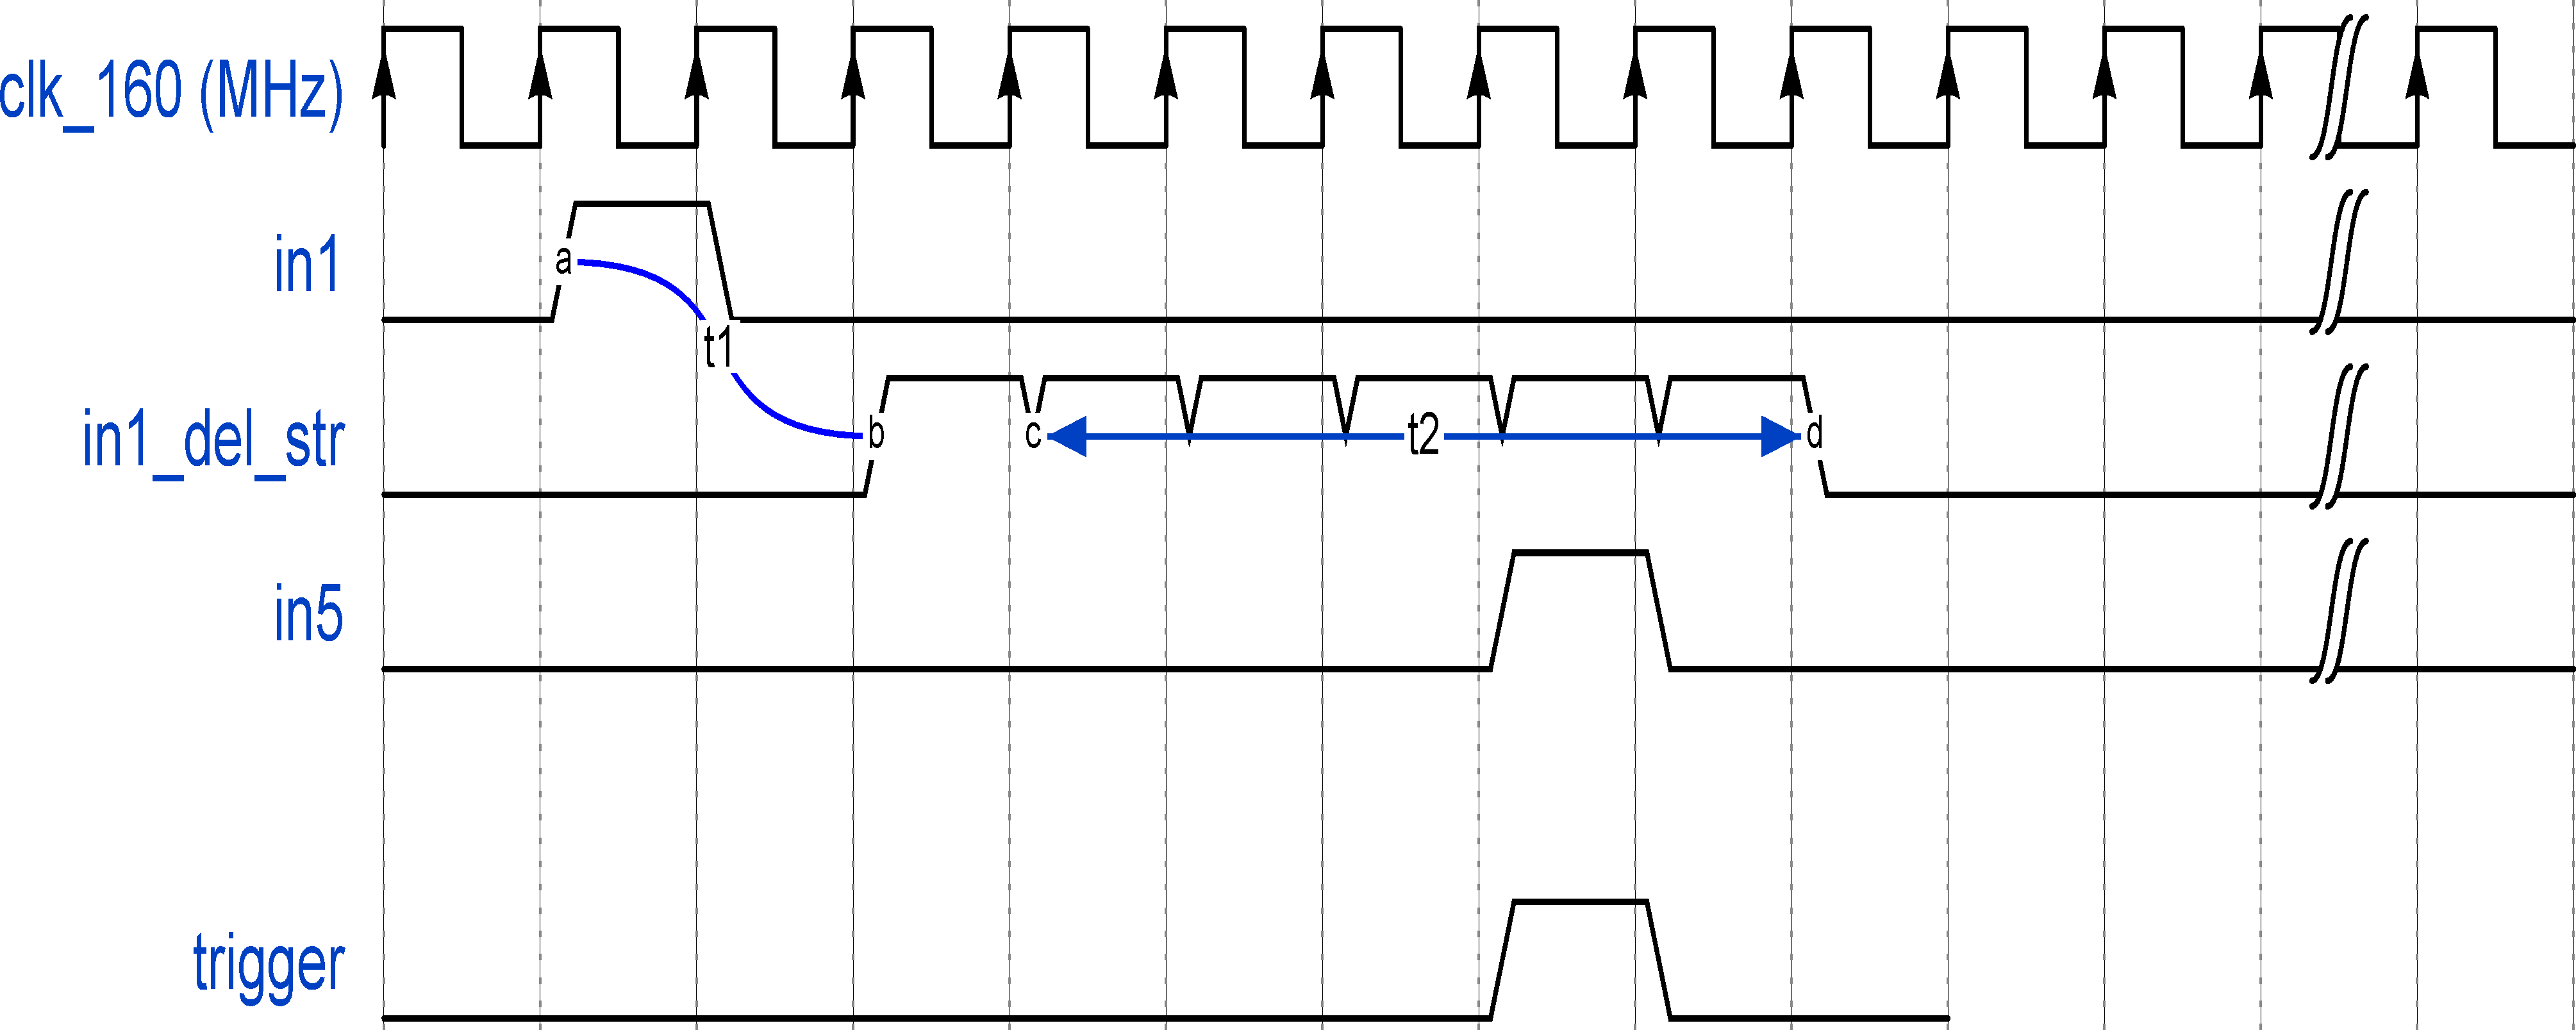
\includegraphics[width=.90\textwidth]{./Images/tlu_trigger_logic.pdf}
  %\includesvg[width=.90\textwidth]{./Images/tlu_trigger_logic.svg}
  \caption{Effect of the stretch and delay values. In1 is delayed by 2 clock cycles (t1= 12.5~ns) and stretched by 5 clock cycles (t2= 31.25~ns) to create a coincidence window with in5 and produce the resulting trigger signal.}
  \label{Fig:trigger_stretchdelay}
\end{figure}\\
 Further details on how to configure the stretch and delay values are provided in section~\ref{ch:EUDAQPar}.
\section{Event buffer}\label{ch:eventBuffer}
The event buffer IPBus slave has four registers.
Writing to \verb|EventFifoCSR| will reset the \gls{fifo}. Reading from either of the register will put their data on the IPBus data line.\\
Reading from \verb|EventFifoCSR| returns the following:
\begin{itemize}
  \item bit 0: \gls{fifo} empty flag
  \item bit 1: \gls{fifo} almost empty flag
  \item bit 2: \gls{fifo} almost full flag
  \item bit 3: \gls{fifo} full flag
  \item bit 4: \gls{fifo} programmable full flag
  \item other bits: 0
\end{itemize}


The status register (SerdesRst) is as follows:
\begin{itemize}
  \item bit 0: reset the ISERDES
  \item bit 1: reset the trigger counters
  \item bit 2: calibrate IDELAY: This seems to be disconnected at the moment.
  \item bit 3: fixed to 0
  \item bit 4, 5: status of \verb|thresholdDeserializer(Input0)|. When the IDELAY modules (prompt, delayed) have reached the correct delay, these two bits should read 00.
  \item bit 6, 7: status of \verb|thresholdDeserializer(Input1)|
  \item bit 8, 9: status of \verb|thresholdDeserializer(Input2)|
  \item bit 10, 11: status of \verb|thresholdDeserializer(Input3)|
  \item bit 12, 13: status of \verb|thresholdDeserializer(Input4)|
  \item bit 14, 15: status of \verb|thresholdDeserializer(Input5)|
  \item bit 16, 19: fixed to 0
  \item bit 20: \verb|s_deserialized_threshold_data(Input0)(7)|
  \item bit 21: \verb|s_deserialized_threshold_data(Input1)(7)|
  \item bit 22: \verb|s_deserialized_threshold_data(Input2)(7)|
  \item bit 23: \verb|s_deserialized_threshold_data(Input3)(7)|
  \item bit 24: \verb|s_deserialized_threshold_data(Input4)(7)|
  \item bit 25: \verb|s_deserialized_threshold_data(Input5)(7)|
  \end{itemize}

9 bits are used to determine trigger edges. 8 are from the deserializers, 1 is added as the LSB and is the MSB from the previous word.

\begin{figure}
  \centering
  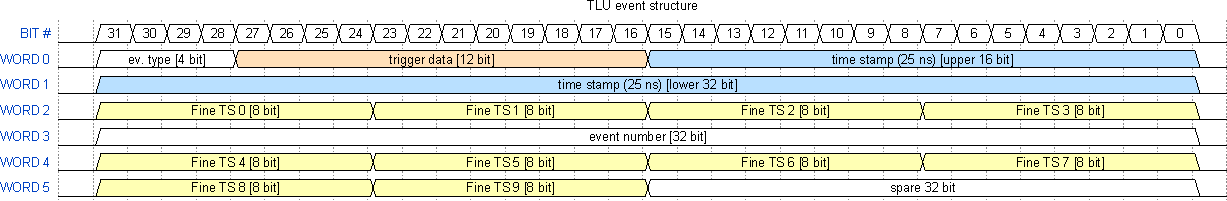
\includegraphics[width=.95\textwidth]{./Images/fifo_words.pdf}
  \caption{Event structure}
  \label{fig:fifo_event}
\end{figure}

\chapter{Appendix}\label{ch:appendix}
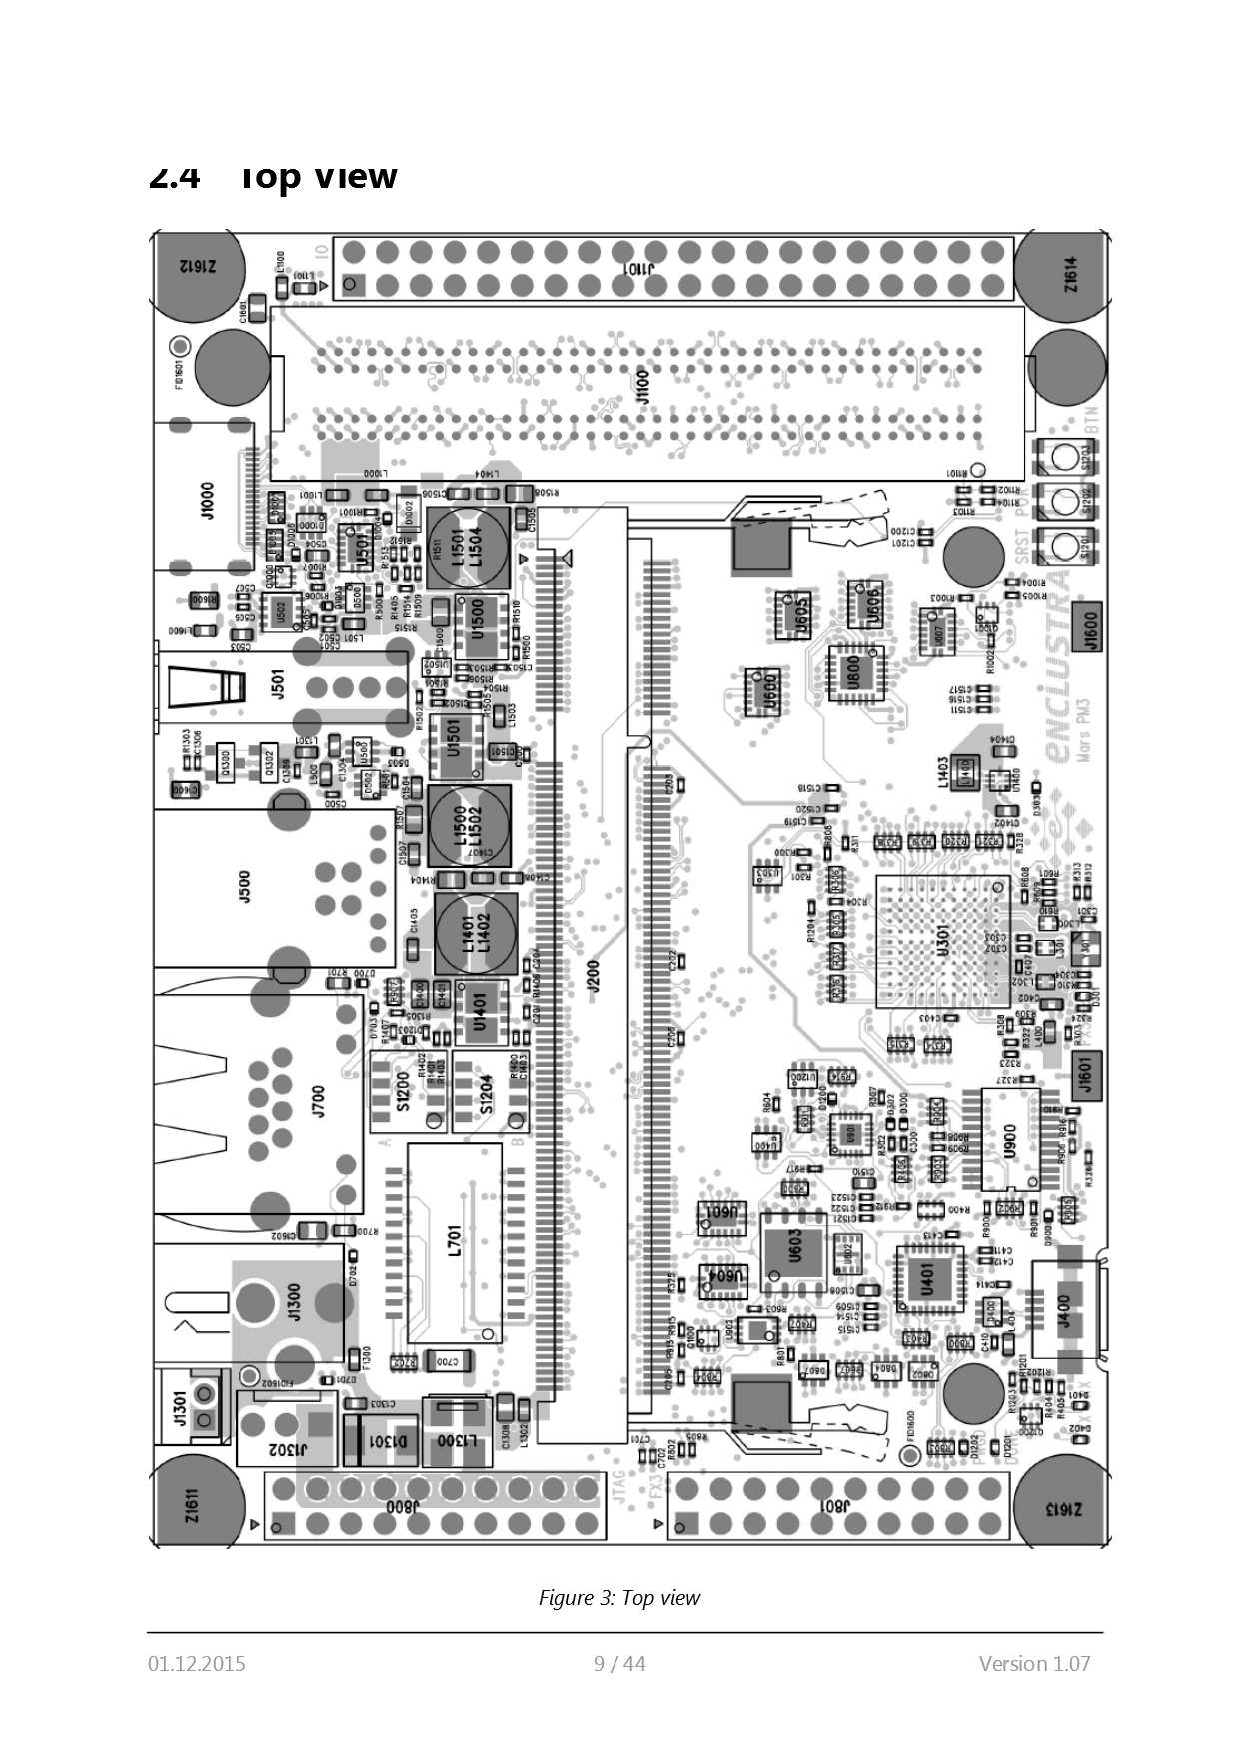
\includepdf[link,pages={1}]{./Docs/PM3TopView.pdf}
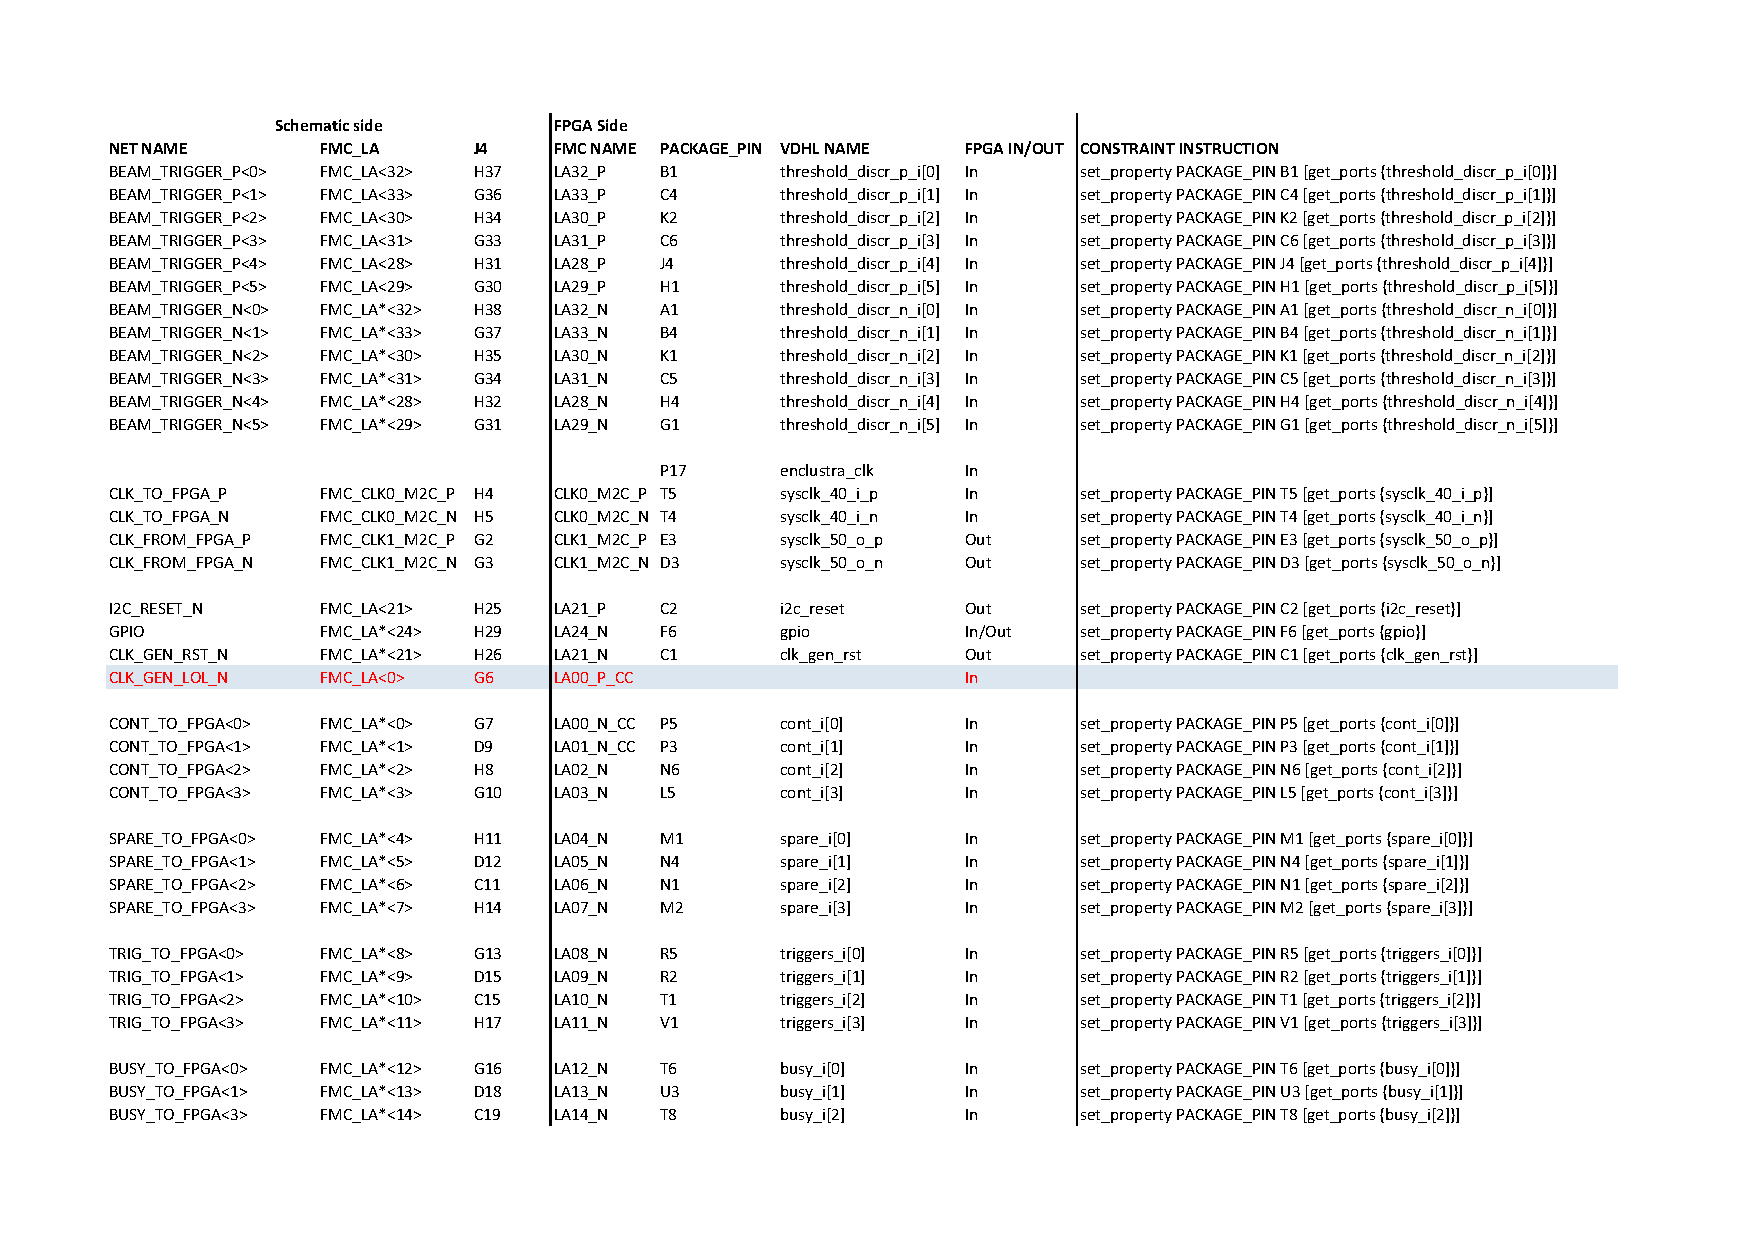
\includepdf[link,pages=-, angle=90]{./Docs/Connections.pdf}
\chapter{Functions}\label{ch:functions}
The following is a list of files containing the code for the \gls{tlu}:
\begin{itemize}
  \item \verb|./eudaq2/user/eudet/misc/fmctlu_runcontrol.ini|:\newline initialization file for the hardware. The location of the file can be passed to the EUDAQ code in the \gls{gui}.
  \item \verb|./eudaq2/user/eudet/misc/fmctlu_runcontrol.conf|:\newline configuration file. It contains all the parameters to be loaded in the \gls{tlu} at the beginning of the run. If this file is not found, EUDAQ will use a list of default settings. The location of the file (and its name) can be passed to the EUDAQ code in the \gls{gui}.
  \item \verb|./eudaq2/user/eudet/misc/fmctlu_connection.xml|:\newline define the IP address and address map of the \gls{tlu}. The one listed is the default location for the file. A different location can be specified with the \verb|ConnectionFile| option in the \emph{conf} file for the \gls{tlu}.
  \item \verb|./eudaq2/user/eudet/misc/fmctlu_address.xml|:\newline address map for the \gls{tlu}. The location of the file is specified in the \verb|fmctlu_connection.xml| file.
  \item \verb|./eudaq2/user/eudet/misc/fmctlu_clock_config.txt|:\newline configuration for the Si5345 clock chip. In order for the hardware to work a configuration file must be present. Those listed are the default name and location for the file; a different file can be specified with the \verb|CLOCK_CFG_FILE| option in the \emph{conf} file for the \gls{tlu}.
  \item \verb|./eudaq2/user/eudet/module/src/FMCTLU_Producer.cc|:\newline eudaq producer for the \gls{tlu}. Contains the methods to initialize, configure, start, stop the \gls{tlu} producer.
  \item \verb|./eudaq2/user/eudet/hardware/src/FmctluController.cc|:\newline Contains the definition of the hardware class for the \gls{tlu} and the methods to set and read from its hardware, such as clock chip, DAC, etc. This lever is abstract with respect to the actual hardware, so that if a future version of the board uses different components it should be possible to re-use this code.
  \item \verb|./eudaq2/user/eudet/hardware/include/FmctluController.hh|:\newline Headers for the controller.
  \item \verb|./eudaq2/user/eudet/hardware/src/FmctluController.cxx|:\newline Executable for the controller.
  \item \verb|./eudaq2/user/eudet/hardware/src/FmctluHardware.cc|:\newline This is the code that deals with the actual hardware on the \gls{tlu}, and contains specific instructions for the chips mounted in the current version. It contains several classes for the ADC, the clock chip, the I/O expanders etc.
  \item \verb|./eudaq2/user/eudet/hardware/include/FmctluHardware.hh|:\newline Header for the hardware.
  \item \verb|./eudaq2/user/eudet/hardware/src/FmctluI2c.cc|:\newline core functions used to read and write from \gls{i2c} compatible slaves.
  \item \verb|./eudaq2/user/eudet/hardware/include/FmctluI2c.hh|:\newline Headers for the \gls{i2c} core.
\end{itemize}

\section{Functions}
\begin{description}
  \item[enableClkLEMO] Enable or disable the output clock to the differential LEMO connector.
  \item[enableHDMI] Set the status of the transceivers for a specific HDMI connector. When enable= False the transceivers are disabled and the connector cannot send signals from FPGA to the outside world. When enable= True then signals from the FPGA will be sent out to the HDMI.\\ In the configuration file use \verb|HDMIx_on = 0| to disable a channel and \verb|HDMI1_on = 1| to enable it (x can be 1, 2, 3, 4).\\
      NOTE: the other direction is always enabled, i.e. signals from the DUTs are always sent to the FPGA.\\
      NOTE: Clock source must be defined separately using SetDutClkSrc (DUTClkSrc in python script).\\
      NOTE: this is called \verb|DUTOutputs| on the python scripts.
  \item[GetFW] dsds
  \item[getSN] dsd
  \item[I2C\_enable] dsd
  \item[InitializeClkChip]
  \item[InitializeDAC]
  \item[InitializeIOexp]
  \item[InitializeI2C]
  \item[PopFrontEvent]
  \item[ReadRRegister]
  \item[ReceiveEvents]
  \item[ResetEventsBuffer]
  \item[SetDutClkSrc] Set the clock source for a specific \gls{hdmi} connector. The source can be set to 0 (no clock), 1 (Si5345) or 2 (FPGA). In the configuration file use \verb|HDMIx_on = N| to select the source (x can be 1, 2, 3, 4, N is the clock source).\\
      NOTE: this is called \verb|DUTClkSrc| on python scripts.
  \item[SetPulseStretchPk] Takes a vector of six numbers, packs them (5-bits each) and sends them to the PulseStretch register.
  \item[SetThresholdValue]
  \item[setTrgPattern] Writes two 32-bit words to define the trigger pattern for the inputs. See section~\ref{ch:triggerinputs} for details.
  \item[SetWRegister]
  \item[SetUhalLogLevel]
\end{description}



\chapter{IPBus Registers}\label{ch:ipbusregs}
%
%\begin{table}[]
%\centering
%\caption{My caption}
%\label{my-label}
%\begin{tabular}{|l|l|r|l|l|l|l|l|}
%\hline
%\textbf{NODE} & \textbf{SUBNODE} & \multicolumn{1}{l|}{\textbf{ADDRESS}} & \textbf{MASK} & \textbf{PERMISSION} & \textbf{DESCRIPTION} & \textbf{MODE} & \textbf{SIZE} \\ \hline
%ID & TLU & \multicolumn{1}{l|}{} &  &  &  &  &  \\ \hline
%\textbf{version} &  & 0x1 &  & r & firmware version &  &  \\
% &  & \multicolumn{1}{l|}{} &  &  &  &  &  \\ \hline
%\textbf{DUTInterfaces} & \textbf{} & \multicolumn{1}{l|}{\textbf{0x1000}} & \textbf{} & \textbf{} & \textbf{DUT Interfaces control registers} & \textbf{} & \textbf{} \\
% & DUTMaskW & 0x0 &  & w &  &  &  \\
% & IgnoreDUTBusyW & 0x1 &  & w &  &  &  \\
% & IgnoreShutterVetoW & 0x2 &  & w &  &  &  \\
% & DUTInterfaceModeW & 0x3 &  & w &  &  &  \\
% & DUTInterfaceModeModifierW & 0x4 &  & w &  &  &  \\
% & DUTInterfaceModeR & 0xB &  & r &  &  &  \\
% & DUTInterfaceModeModifierR & 0xC &  & r &  &  &  \\
% & DUTMaskR & 0x8 &  & r &  &  &  \\
% & IgnoreDUTBusyR & 0x9 &  & r &  &  &  \\
% & IgnoreShutterVetoR & 0xA &  & r &  &  &  \\
% &  & \multicolumn{1}{l|}{} &  &  &  &  &  \\ \hline
%\textbf{Shutter} &  & \multicolumn{1}{l|}{\textbf{0x2000}} & \textbf{} & \textbf{} & \textbf{Shutter/T0 control} & \textbf{} &  \\
% & ShutterStateW & 0x0 &  & w &  &  &  \\
% & PulseT0 & 0x1 &  & w &  &  &  \\
% &  & \multicolumn{1}{l|}{} &  &  &  &  &  \\ \hline
%\textbf{i2c\_master} & \textbf{} & \multicolumn{1}{l|}{\textbf{0x3000}} & \textbf{} & \textbf{} & \textbf{I2C Master interface} & \textbf{} & \textbf{} \\
% & i2c\_pre\_lo & 0x0 & 0xFF & r/w &  &  &  \\
% & i2c\_pre\_hi & 0x1 & 0xFF & r/w &  &  &  \\
% & i2c\_ctrl & 0x2 & 0xFF & r/w &  &  &  \\
% & i2c\_rxtx & 0x3 & 0xFF & r/w &  &  &  \\
% & i2c\_cmdstatus & 0x4 & 0xFF & r/w &  &  &  \\
% &  & \multicolumn{1}{l|}{} &  &  &  &  &  \\ \hline
%\textbf{eventBuffer} & \textbf{} & \multicolumn{1}{l|}{\textbf{0x4000}} & \textbf{} & \textbf{} & \textbf{Event buffer} & \textbf{} & \textbf{} \\
% & EventFifoData & 0x0 &  & r &  & non-incremental & 3200 \\
% & EventFifoFillLevel & 0x1 &  & r &  &  &  \\
% & EventFifoCSR & 0x2 &  & r/w &  &  &  \\
% & EventFifoFillLevelFlags & 0x3 &  & r &  &  &  \\
% &  & \multicolumn{1}{l|}{} &  &  &  &  &  \\ \hline
%\textbf{Event\_Formatter} & \textbf{} & \multicolumn{1}{l|}{\textbf{0x5000}} & \textbf{} & \textbf{} & \textbf{Event formatter configuration} & \textbf{} & \textbf{} \\
% & Enable\_Record\_Data & 0x0 &  & r/w &  &  &  \\
% & ResetTimestampW & 0x1 &  & w &  &  &  \\
% & CurrentTimestampLR & 0x2 &  & r &  &  &  \\
% & CurrentTimestampHR & 0x3 &  & r &  &  &  \\
% &  & \multicolumn{1}{l|}{} &  &  &  &  &  \\ \hline
%\textbf{triggerInputs} & \textbf{} & \multicolumn{1}{l|}{\textbf{0x6000}} & \textbf{} & \textbf{} & \textbf{Inputs configuration} & \textbf{} & \textbf{} \\
% & SerdesRstW & 0x0 &  & w &  &  &  \\
% & SerdesRstR & 0x8 &  & r &  &  &  \\
% & ThrCount0R & 0x9 &  & r &  &  &  \\
% & ThrCount1R & 0xA &  & r &  &  &  \\
% & ThrCount2R & 0xB &  & r &  &  &  \\
% & ThrCount3R & 0xC &  & r &  &  &  \\
% & ThrCount4R & 0xD &  & r &  &  &  \\
% & ThrCount5R & 0xE &  & r &  &  &  \\
% &  & \multicolumn{1}{l|}{} &  &  &  &  &  \\ \hline
%\textbf{triggerLogic} & \textbf{} & \multicolumn{1}{l|}{\textbf{0x7000}} & \textbf{} & \textbf{} & \textbf{Trigger logic configuration} & \textbf{} & \textbf{} \\
% & PostVetoTriggersR & 0x10 &  & r &  &  &  \\
% & PreVetoTriggersR & 0x11 &  & r &  &  &  \\
% & InternalTriggerIntervalW & 0x02 &  & w &  &  &  \\
% & InternalTriggerIntervalR & 0x12 &  & r &  &  &  \\
% & TriggerVetoW & 0x04 &  & w &  &  &  \\
% & TriggerVetoR & 0x14 &  & r &  &  &  \\
% & ExternalTriggerVetoR & 0x15 &  & r &  &  &  \\
% & PulseStretchW & 0x06 &  & w &  &  &  \\
% & PulseStretchR & 0x16 &  & r &  &  &  \\
% & PulseDelayW & 0x07 &  & w &  &  &  \\
% & PulseDelayR & 0x17 &  & r &  &  &  \\
% & TriggerHoldOffW & 0x08 &  & w &  &  &  \\
% & TriggerHoldOffR & 0x18 &  & r &  &  &  \\
% & AuxTriggerCountR & 0x19 &  & r &  &  &  \\
% & TriggerPattern\_lowW & 0x0A &  & w &  &  &  \\
% & TriggerPattern\_lowR & 0x1A &  & r &  &  &  \\
% & TriggerPattern\_highW & 0x0B &  & w &  &  &  \\
% & TriggerPattern\_highR & 0x1B &  & r &  &  &  \\
% &  & \multicolumn{1}{l|}{} &  &  &  &  &  \\ \hline
%\textbf{logic\_clocks} & \textbf{} & \multicolumn{1}{l|}{\textbf{0x8000}} & \textbf{} & \textbf{} & \textbf{Clocks configuration} & \textbf{} & \textbf{} \\
% & LogicClocksCSR & 0x0 &  & r/w &  &  &  \\
% & LogicRst & 0x1 &  & w &  &  &  \\ \hline
%\end{tabular}
%\end{table}

\begin{table}
\centering
\footnotesize
\caption{IPBus register}
\label{tab:ipbusreg}
\begin{tabular}{|l|l|r|l|l|}
\hline
\textbf{NODE} & \textbf{SUBNODE} & \multicolumn{1}{l|}{\textbf{ADDRESS}} & \textbf{MASK} & \textbf{PERMISSION} \\ \hline
\textbf{version} &  & 0x1 &  & r \\ \hline
\textbf{DUTInterfaces} & \textbf{} & \multicolumn{1}{l|}{\textbf{0x1000}} & \textbf{} & \textbf{} \\
 & DUTMaskW & 0x0 &  & w \\
 & IgnoreDUTBusyW & 0x1 &  & w \\
 & IgnoreShutterVetoW & 0x2 &  & w \\
 & DUTInterfaceModeW & 0x3 &  & w \\
 & DUTInterfaceModeModifierW & 0x4 &  & w \\
 & DUTInterfaceModeR & 0xB &  & r \\
 & DUTInterfaceModeModifierR & 0xC &  & r \\
 & DUTMaskR & 0x8 &  & r \\
 & IgnoreDUTBusyR & 0x9 &  & r \\
 & IgnoreShutterVetoR & 0xA &  & r \\ \hline
\textbf{Shutter} &  & \multicolumn{1}{l|}{\textbf{0x2000}} & \textbf{} & \textbf{} \\
 & ShutterStateW & 0x0 &  & w \\
 & PulseT0 & 0x1 &  & w \\ \hline
\textbf{i2c\_master} & \textbf{} & \multicolumn{1}{l|}{\textbf{0x3000}} & \textbf{} & \textbf{} \\
 & i2c\_pre\_lo & 0x0 & 0xFF & r/w \\
 & i2c\_pre\_hi & 0x1 & 0xFF & r/w \\
 & i2c\_ctrl & 0x2 & 0xFF & r/w \\
 & i2c\_rxtx & 0x3 & 0xFF & r/w \\
 & i2c\_cmdstatus & 0x4 & 0xFF & r/w \\ \hline
\textbf{eventBuffer} & \textbf{} & \multicolumn{1}{l|}{\textbf{0x4000}} & \textbf{} & \textbf{} \\
 & EventFifoData & 0x0 &  & r \\
 & EventFifoFillLevel & 0x1 &  & r \\
 & EventFifoCSR & 0x2 &  & r/w \\
 & EventFifoFillLevelFlags & 0x3 &  & r \\ \hline
\textbf{Event\_Formatter} & \textbf{} & \multicolumn{1}{l|}{\textbf{0x5000}} & \textbf{} & \textbf{} \\
 & Enable\_Record\_Data & 0x0 &  & r/w \\
 & ResetTimestampW & 0x1 &  & w \\
 & CurrentTimestampLR & 0x2 &  & r \\
 & CurrentTimestampHR & 0x3 &  & r \\ \hline
\textbf{triggerInputs} & \textbf{} & \multicolumn{1}{l|}{\textbf{0x6000}} & \textbf{} & \textbf{} \\
 & SerdesRstW & 0x0 &  & w \\
 & SerdesRstR & 0x8 &  & r \\
 & ThrCount0R & 0x9 &  & r \\
 & ThrCount1R & 0xA &  & r \\
 & ThrCount2R & 0xB &  & r \\
 & ThrCount3R & 0xC &  & r \\
 & ThrCount4R & 0xD &  & r \\
 & ThrCount5R & 0xE &  & r \\ \hline
\textbf{triggerLogic} & \textbf{} & \multicolumn{1}{l|}{\textbf{0x7000}} & \textbf{} & \textbf{} \\
 & PostVetoTriggersR & 0x10 &  & r \\
 & PreVetoTriggersR & 0x11 &  & r \\
 & InternalTriggerIntervalW & 0x02 &  & w \\
 & InternalTriggerIntervalR & 0x12 &  & r \\
 & TriggerVetoW & 0x04 &  & w \\
 & TriggerVetoR & 0x14 &  & r \\
 & ExternalTriggerVetoR & 0x15 &  & r \\
 & PulseStretchW & 0x06 &  & w \\
 & PulseStretchR & 0x16 &  & r \\
 & PulseDelayW & 0x07 &  & w \\
 & PulseDelayR & 0x17 &  & r \\
 & TriggerHoldOffW & 0x08 &  & w \\
 & TriggerHoldOffR & 0x18 &  & r \\
 & AuxTriggerCountR & 0x19 &  & r \\
 & TriggerPattern\_lowW & 0x0A &  & w \\
 & TriggerPattern\_lowR & 0x1A &  & r \\
 & TriggerPattern\_highW & 0x0B &  & w \\
 & TriggerPattern\_highR & 0x1B &  & r \\ \hline
\textbf{logic\_clocks} & \textbf{} & \multicolumn{1}{l|}{\textbf{0x8000}} & \textbf{} & \textbf{} \\
 & LogicClocksCSR & 0x0 &  & r/w \\
 & LogicRst & 0x1 &  & w \\ \hline
\end{tabular}
\end{table}

\begin{description}
  \item[version] Returns the current version of firmware used to program the \gls{tlu}
  \item[------------------------]
  \item[DUTINTERFACES]
  \item[DUTMaskW] Writing to this register allows to define which \gls{dut}s are active when in AIDA mode. The lower 4 bits of the register can be used to define the status of the \gls{dut}s: 1 for active, 0 for masked. \verb|hdmi1| is defined by bit 0, \verb|hdmi2| is defined by bit 1, \verb|hdmi3| is defined by bit 2, \verb|hdmi4| is defined by bit 3.
  \item[IgnoreDUTBusyW] Writing to this register allows to ignore the busy signal from a particular \gls{dut} while in AIDA mode. The lower 4 bits are used to define the status for each device. A 1 indicates that the logic should ignore busy signals from the specific \gls{dut}.
  \item[IgnoreShutterVetoW] The \gls{lsb} of this register can be written to define whether the \gls{dut} should ignore the shutter veto signal. Normally, when the shutter signal is asserted the \gls{dut} reports busy. If this bit is flag the \gls{dut} will ignore the shutter signal.
  \item[DUTInterfaceModeW] Write register to define the mode of operation for a \gls{dut}. Two bits per device can be used to define the mode; currently only two modes are available (AIDA, EUDET).\\
      The bit pairs are packed from the \gls{lsb} starting with \verb|hdmi1| (bits 0, 1), \verb|hdmi2| (bits 2, 3), \verb|hdmi3| (bits 4, 5),  \verb|hdmi4| (bits 6, 7).
      \begin{itemize}
        \item bit pair X0: EUDET
        \item bit pair X1: AIDA
      \end{itemize}
  \item[DUTInterfaceModeModifierW] Write register. This register only affects the EUDET mode of operation. For each \gls{dut} two bits can be configured although cyrrently only the lower of the pair is considere. The bit packing is done in a manner similar to the DUTInterfaceMode. Set bit high to allow asynchronous veto using \verb|DUT_CLK| when in EUDET mode.
  \item[DUTInterfaceModeR] Read the content of the DUTInterfaceMode register.
  \item[DUTInterfaceModeModifierR] Read status of the DUTInterfaceMode register.
  \item[DUTMaskR] Read the status of the DUTMask register.
  \item[IgnoreDUTBusyR] Read the status of the IgnoreDUTBusy register.
  \item[IgnoreShutterVetoR] Read the status of the IgnoreShutterVeto word (only the last bit is meanigful).
\end{description}

\begin{description}
  \item[------------------------]
  \item[SHUTTER]
  \item[ShutterStateW] The \gls{lsb} of this register is propagated to the \gls{dut}s as shutter signal. This is the signal that the \gls{dut}s receive on the \verb|cont| line.
  \item[PulseT0] Writing to this register will cause the firmware to generate a T0 signal.
\end{description}

\begin{description}
  \item[------------------------]
  \item[I2C\_MASTER] This section includes registers used to talk to the \gls{i2c} bus.
  \item[i2c\_pre\_lo] Lower part of the clock pre-scaler value. The pre-scaler is used to reduce the clock frequency of the bus and make it compatible with the \gls{i2c} slaves on the board.
  \item[i2c\_pre\_hi] Higher part of the clock pre-scaler value.
  \item[i2c\_ctrl]
  \item[i2c\_rxtx]
  \item[i2c\_cmdstatus]
\end{description}

\begin{description}
  \item[------------------------]
  \item[EVENTBUFFER]
  \item[EventFifoData]      Returns the content of the \gls{fifo}. In the current firmware implementation the memory can hold 8192 words (32-bit).
  \item[EventFifoFillLevel] Read register. Returns the number of words written in the \gls{fifo}. The lowest 14-bits are the actual data.
  \item[EventFifoCSR]       Read or write register. When read it returns the status of the \gls{fifo}. Five flags are returned:
                              \begin{itemize}
                                \item bit 0: empty. Asserted when the \gls{fifo} is empty.
                                \item bit 1: almost empty. Asserted when one word remains in the \gls{fifo}.
                                \item bit 2: almost full. Asserted when the \gls{fifo} can only accept one more word before becoming full.
                                \item bit 3: full. In the current firmware the \gls{fifo} can hold 8192 words before filling up.
                                \item bit 4: programmable full. This signal is asserted when the number of words in the FIFO is greater than or equal to the assert threshold (8181). It is de-asserted when the number of words in the FIFO is less than the negate threshold (8180).
                              \end{itemize}
                                When any value is written to this register the \gls{fifo} is reset.
  \item[EventFifoFillLevelFlags] Does not do anything? REMOVE \textcolor[rgb]{1.00,0.00,0.00}{CHECK}
\end{description}

\begin{description}
  \item[------------------------]
  \item[EVENT\_FORMATTER]
  \item[Enable\_Record\_Data] Read and write register. When written, \textcolor[rgb]{1.00,0.00,0.00}{CHECK}\\
                                When read returns the content of the enable record word.
  \item[ResetTimestampW]        Write register. Writing any value to this register will cause the firmware to produce a retest timestamp signal (high for one clock cycle of clk\_4x\_logic). At the moment it does not seems to be connected to anything. \textcolor[rgb]{1.00,0.00,0.00}{CHECK}
  \item[CurrentTimestampLR] \textcolor[rgb]{1.00,0.00,0.00}{CHECK}
  \item[CurrentTimestampHR] \textcolor[rgb]{1.00,0.00,0.00}{CHECK}
\end{description}

\begin{description}
  \item[------------------------]
  \item[TRIGGERINPUTS]
  \item[SerdesRstW] Write register for the SerDes control.\begin{itemize}
                                                            \item bit 0: set this bit to reset the ISERDES
                                                            \item bit 1: set this bit to reset the input trigger counters
                                                            \item bit 2: \verb|s_calibrate_delay|
                                                          \end{itemize}
  \item[SerdesRstR] Read register for the SerDes control.
  \item[ThrCount0R] Read register. Returns the number of pulses above threshold for the trigger input.
  \item[ThrCount1R] Read register. Returns the number of pulses above threshold for the trigger input.
  \item[ThrCount2R] Read register. Returns the number of pulses above threshold for the trigger input.
  \item[ThrCount3R] Read register. Returns the number of pulses above threshold for the trigger input.
  \item[ThrCount4R] Read register. Returns the number of pulses above threshold for the trigger input.
  \item[ThrCount5R] Read register. Returns the number of pulses above threshold for the trigger input.
\end{description}

\begin{description}\label{ch:triggerLogic}
  \item[------------------------]
  \item[TRIGGERLOGIC]
  \item[PostVetoTriggersR] Read register. Returns the number of triggers recorded in the \gls{tlu} after the veto is applied. These are the triggers actually sent to the \gls{dut}s.
  \item[PreVetoTriggersR] Read register. Returns the number of triggers recorded in the \gls{tlu} before the veto is applied. This is used for debugging purposes.
  \item[InternalTriggerIntervalW] Write the number of clock cycles to be used as period for the internal trigger generator. If this number is smaller than 5 then the triggers are disabled. Otherwise the period is number -2.
  \item[InternalTriggerIntervalR] Read the value written in InternalTriggerIntervalW.
  \item[TriggerVetoW] Write register. The value written to the \gls{lsb} of this register is used to generate a veto signal. This can be used to put switch the \gls{tlu} status: if the bit is asserted the logic will not send new triggers to the \gls{dut}s. If the bit is reset the board will process new triggers.
  \item[TriggerVetoR] Read the content of the TriggerVeto register.
  \item[ExternalTriggerVetoR] Read register. Bit 0 of this register reports the \verb|veto| status (1 for veto active, 0 for no veto). The veto is active if the \gls{tlu} buffer is full or if one of the \gls{dut}s is sending a veto signal.
  \item[PulseStretchW] Write the stretch word for the trigger pulses. The original trigger pulses collected at a trigger input can be stretched by $N$ cycles of the 4x clock (160~MHz, 6.25~ns). $N$ is a number between 0 and 31. The stretched pulse is always at least as long as the original input.\\
      The stretch values can be written in the \verb|conf| file using the parameters \verb|inX_STR| (X= [0 ... 5]).\\
      The six words for the inputs are packed in a single 32-bit word written to this register according to the format shown in table~\ref{tab:packing}.
  \item[PulseStretchR] Returns the content of the PulseStretch word.
  \item[PulseDelayW] Write the delay word for the trigger pulses. The original pulse is delayed by $N$ clycles of the 4x clock (160~MHz, 6.25~ns). $N$ is a number between 0 and 31. The six words for the inputs are packed in a single 32-bit word written to this register according to the format shown in table~\ref{tab:packing}.\\
      The delay values can be written in the \verb|conf| file using the parameters \verb|inX_DEL| (X= [0 ... 5]).\\
  \item[PulseDelayR] Returns the content of the PulseDelay word.
  \item[TriggerHoldOffW] Does not do anything? \textcolor[rgb]{1.00,0.00,0.00}{CHECK}
  \item[TriggerHoldOffR] Read the previous register... \textcolor[rgb]{1.00,0.00,0.00}{CHECK}
  \item[AuxTriggerCountR] Auxiliary trigger counter. Used for debug.
  \item[TriggerPattern\_lowW] Write register for the lower 32-bits of the trigger pattern. This pattern is used to select the combinations of trigger signals that produce a valid trigger in the \gls{tlu}. See section~\ref{ch:triggerLogic} for details.
  \item[TriggerPattern\_lowR] Read register for the lower 32-bits of the trigger pattern. This pattern is used to select the combinations of trigger signals that produce a valid trigger in the \gls{tlu}. See section~\ref{ch:triggerLogic} for details.
  \item[TriggerPattern\_highW] Write register for the higher 32-bits of the trigger pattern. This pattern is used to select the combinations of trigger signals that produce a valid trigger in the \gls{tlu}. See section~\ref{ch:triggerLogic} for details.
  \item[TriggerPattern\_highR] Read register for the higher 32-bits of the trigger pattern. This pattern is used to select the combinations of trigger signals that produce a valid trigger in the \gls{tlu}. See section~\ref{ch:triggerLogic} for details.
\end{description}

\begin{description}
  \item[------------------------]
  \item[LOGIC\_CLOCKS]
  \item[LogicClocksCSR] This is a read/write register. The write function is now obsolete and should be removed. Reading from this register returns the status of the PLL lock: bit 0 is the locked value of the pll (1= locked).
  \item[LogicRst] Writing a 1 in the LSB of this register will reset the PLL and the clocks used by the \gls{tlu} firmware. It needs to be checked for bugs.
\end{description}

\begin{sidewaystable}[]
\footnotesize
    \caption{Packing scheme for values in registers used to define the pulse stretch and delay.}
    \label{tab:packing}
    \begin{tabular}{|l|l|l|l|l|l|l|l|l|l|l|l|l|l|l|l|l|l|l|l|l|l|l|l|l|l|l|l|l|l|l|l|}
    \hline
    \multicolumn{32}{|c|}{Register value}                                                                                                                                                             \\ \hline
    31 & 30 & 29   & 28  & 27  & 26  & 25  & 24   & 23  & 22  & 21  & 20  & 19   & 18  & 17  & 16  & 15  & 14   & 13  & 12  & 11  & 10  & 9    & 8   & 7   & 6   & 5   & 4    & 3   & 2   & 1   & 0   \\ \hline
    x  & x  & \multicolumn{5}{c|}{Input 5} & \multicolumn{5}{c|}{Input 4} & \multicolumn{5}{c|}{Input 3} & \multicolumn{5}{c|}{Input 2} & \multicolumn{5}{c|}{Input 1} & \multicolumn{5}{c|}{Input 0} \\ \hline
    x  & x  & b4   & b3  & b2  & b1  & b0  & b4   & b3  & b2  & b1  & b0  & b4   & b3  & b2  & b1  & b0  & b4   & b3  & b2  & b1  & b0  & b4   & b3  & b2  & b1  & b0  & b4   & b3  & b2  & b1  & b0  \\ \hline
    \end{tabular}
\end{sidewaystable}

\chapter{EUDAQ Parameters}\label{ch:EUDAQPar}
List of parameters that are parsed by the EUDAQ run control \gls{gui} to configure the \gls{tlu}.\\
The parameters must be included in the INI or CONF file passed to the main window (see~fig.\ref{fig:EUDAQGui}).
\begin{figure}
  \centering
  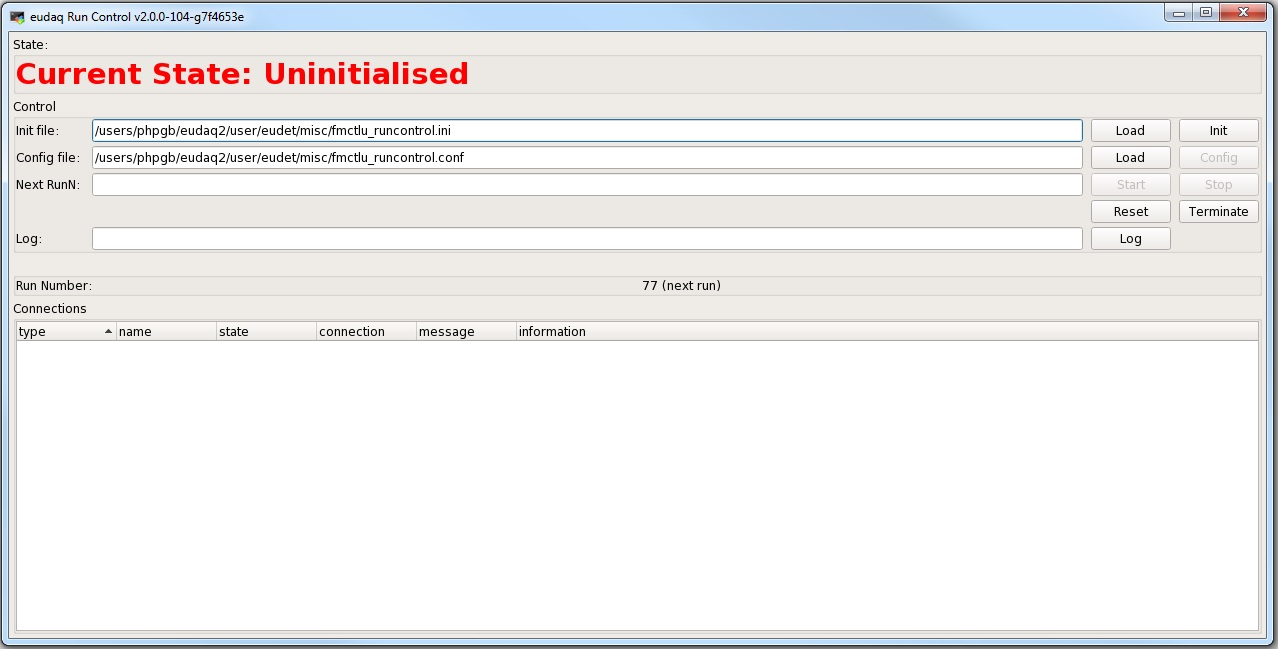
\includegraphics[width=.90\textwidth]{./Images/RunControlGUI.jpg}
  \caption{Main user iterface of the EUDAQ framework.}
  \label{fig:EUDAQGui}
\end{figure}\\
Not all parameters are needed; if one of the parameters is not present in the files, the code will generally assume a default value, indicated in brackets in the following document \verb|[type, default]|.
\section{INI file}
\begin{description}
  \item[initid] \verb|[string, "0"]| Does not serve any purpose in the code but can be useful to identify configuration settings used in a specific run. EUDAQ will store this information in the run data.
  \item[ConnectionFile] \verb|[string, "file://./FMCTLU_connections.xml"]| Name of the xml file used to store the information required to communicate with the hardware, such as its IP address and the location of the address map. The default location indicates a file that must be located in the \texttt{bin} folder.
  \item[DeviceName] \verb|[string, "fmctlu.udp"]| The name of the type of hardware to be contacted by the IPBus.
  \item[TLUmod] \verb|[string, "1e"]| Version of the \gls{tlu} hardware. Reserved for future use.
  \item[nDUTs] \verb|[positive int, 4]| Number of \gls{dut} in the current \gls{tlu}. This is for future upgrades and should not require editing by the user.
  \item[nTrgIn] \verb|[positive int, 6]| Number of trigger inputs in the current \gls{tlu}. This is for future upgrades and should not require editing by the user.
  \item[I2C\_COREEXP\_Addr] \verb|[positive int, 0x21]| \gls{i2c} address of the core expander mounted on the Enclustra board. This is not required if a different \gls{fpga} is used. See section~\ref{ch:i2c} for further details.
  \item[I2C\_CLK\_Addr] \verb|[positive int, 0x68]| \gls{i2c} address of Si5345 clock generator installed on the \gls{tlu}.
  \item[I2C\_DAC1\_Addr] \verb|[positive int, 0x13]| \gls{i2c} address of \gls{dac} installed on the \gls{tlu}. The \gls{dac} is used to configure the threshold of the trigger inputs.
  \item[I2C\_DAC2\_Addr] \verb|[positive int, 0x1F]| \gls{i2c} address of \gls{dac} installed on the \gls{tlu}. The \gls{dac} is used to configure the threshold of the trigger inputs.
  \item[I2C\_ID\_Addr] \verb|[positive int, 0x50]| \gls{i2c} address the unique ID \gls{eeprom} installed on the \gls{tlu}. The chip is used to provide a unique identifier to each kit.
  \item[I2C\_EXP1\_Addr] \verb|[positive int, 0x74]| \gls{i2c} address the bus expander used to select the direction of the \gls{hdmi} pins on the board.
  \item[I2C\_EXP2\_Addr] \verb|[positive int, 0x75]| \gls{i2c} address the bus expander used to select the direction of the \gls{hdmi} pins on the board.
  \item[intRefOn] \verb|[boolean, false]| If true, the \gls{dac}s installed on the \gls{tlu} will use their internal voltage reference rather than the one provide externally.
  \item[VRefInt] \verb|[float, 2.5]| Value in volts for the internal reference voltage of the \gls{dac}s. The voltage is chosen by the chip manufacturer. This is only used if \verb|intRefOn= true|.
  \item[VRefExt] \verb|[float, 1.3]| Value in volts for the external reference voltage of the \gls{dac}s. The voltage is determined by a circuit on the \gls{tlu} and the value of this parameter must reflect such voltage. This is only used if \verb|intRefOn= false|.
  \item[CONFCLOCK] \verb|[boolean, true]| If true, the clock chip Si5345 will be re-configured when the INIT button is pressed (see figure~fig.\ref{fig:EUDAQGui}). The chip is configured via \gls{i2c} interface using a specific text file (see next parameter). After a power cycle, the chip is not configured and must be reconfigured to operate the \gls{tlu} correctly.
  \item[CLOCK\_CFG\_FILE] \verb|[string, "./../user/eudet/misc/fmctlu_clock_config.txt"]| Name of the text file used to store the configuration values of the Si5345. The file can be generate using the Clockbuilder Pro software provided by \href{https://www.silabs.com/products/development-tools/software/clock}{SiLabs}.
\end{description}

\section{CONF file}
\begin{description}
  \item[confid] \verb|[string, "0"]| Does not serve any purpose in the code but can be useful to identify configuration settings used in a specific run. EUDAQ will store this information in the run data.
  \item[verbose] \verb|[int, 0]| Defines the level of output messages from the \gls{tlu}. 0 indicates minimum output.
  \item[HDMI1\_set] \verb|[unsigned int, 0b0001]| Defines the source of the signal on the pins for the \verb|HDMI1| connector. A 1 indicates that each pin pair is an driven by the \gls{tlu}, a 0 that they are left floating (with respect to the \gls{tlu}). This can be used to define the signal direction on each pin pair. The order of the pairs is as follow:\\
  bit 0= CONT, bit 1= SPARE, bit 2= TRIG, trig 3= BUSY. Note that the direction of the DUTClk pair is defined in a separate parameter.\\
  Example to configure the connector to work with an EUDET device:\\
  - in this configuration the BUSY line is driven by the device under test, so it is an input for the \gls{tlu} and should not be driven by it (bit 3= 0)\\
  - TRIGGER line is an output for the \gls{tlu} so is driven by it (bit 2= 1)\\
  - SPARE line is used to provide control signals, such as the reset signal to initialize the devices at the start of a run (\texttt{T$_0$}). It should be configured as driven by the \gls{tlu} (bit 1= 1)\\
  - CONT is used by the \gls{tlu} to issue control commands and should be configured as a signal driven by the \gls{tlu} (bit 0= 1).\\
  Therefore the value of this parameter would be 0x7 (b1110).
  \item[HDMI2\_set] \verb|[unsigned int, 0b0001]| Defines the direction of the pins for the \verb|HDMI2| connector.
  \item[HDMI3\_set] \verb|[unsigned int, 0b0001]| Defines the direction of the pins for the \verb|HDMI3| connector.
  \item[HDMI4\_set] \verb|[unsigned int, 0b0001]| Defines the direction of the pins for the \verb|HDMI4| connector.
  \item[HDMI1\_clk] \verb|[unsigned int, 1]| Defines if the DUTClk pair on the \gls{hdmi} connector must be driven by the \gls{tlu} and, if so, what clock source to use. A 0 indicates that the pins are not driven by the \gls{tlu}. 1 indicates that pins will by driven with the clock produced from the on-board clock chip Si5345. 2 indicates that the driving clock is obtained from the \gls{fpga}.\\
      Example to configure the connector to work with an EUDET device: in this scenario the clock is driven by the \gls{dut} so the parameter should be set to 0.
      Example to configure the connector to work with an AIDA device: in this scenario the clock is driven by the \gls{tlu} so the parameter should be set to either 1 or 2 (by default 1).
  \item[HDMI2\_clk] \verb|[unsigned int, 1]| Defines the driving signal on the corresponding \gls{hdmi} connector.
  \item[HDMI3\_clk] \verb|[unsigned int, 1]| Defines the driving signal on the corresponding \gls{hdmi} connector.
  \item[HDMI4\_clk] \verb|[unsigned int, 1]| Defines the driving signal on the corresponding \gls{hdmi} connector.
  \item[LEMOclk] \verb|[boolean, true]| Defines whether a driving clock is to be provided on the differential LEMO connector of the \gls{tlu}. By default (value= 1), the clock is driven from the clock chip. If the value is set to 0 no clock will be driven.
  \item[in0\_STR] \verb|[unsigned int, 0]| Defines the number of clock cycles used to stretch a pulse once a trigger is detected by the discriminator on input 0. This feature allows the user to modify the pulses that are then fed into the trigger logic within the \gls{tlu}.
      A minimum lenght of 6.25~ns is provided if the value is 0. Any extra clock cycle extend the pulse by 6.25~ns (160~MHz clock). An example of the effect on the stretch setting is shown in figure~\ref{Fig:exampleExtendedTriggers}.
  \item[in0\_DEL] \verb|[unsigned int, 0]| Defines the delay, in 160~MHz clock cycles, to be assigned to the discriminated pulse from input 0, in order to process the logic for the trigger. This can be used to compensate for differences in cable lengths for the signals used to create a trigger.
  \item[in1\_STR] \verb|[unsigned int, 0]| Same as \texttt{in1\_STR} but for input 1.
  \item[in1\_DEL] \verb|[unsigned int, 0]| Same as \texttt{in1\_DEL} but for input 1.
  \item[in2\_STR] \verb|[unsigned int, 0]| Same as \texttt{in1\_STR} but for input 2.
  \item[in2\_DEL] \verb|[unsigned int, 0]| Same as \texttt{in1\_DEL} but for input 1.
  \item[in3\_STR] \verb|[unsigned int, 0]| Same as \texttt{in1\_STR} but for input 3.
  \item[in3\_DEL] \verb|[unsigned int, 0]| Same as \texttt{in1\_DEL} but for input 1.
  \item[trigMaskHi] \verb|[unsigned int32, 0]| This word represents the most significative bits of the 64-bits used to determine the trigger mask.\\
        A detailed explanation of how to determine the correct word is provided in section~\ref{ch:triggerLogic}.
  \item[trigMaskLo] \verb|[unsigned int32, 0]| This word represents the least significative bits of the 64-bits used to determine the trigger mask.\\
        A detailed explanation of how to determine the correct word is provided in section~\ref{ch:triggerLogic}.
  \item[DUTMask]  \verb|[unsigned int, 0x1]| This mask indicates which \gls{hdmi} inputs have an AIDA device connected. Each of the lowest four bits correspond to a connector (bit 0= DUT1, bit 1= DUT2, bit 2= DUT3, bit 3= DUT4). If the bit is set to 1 the \gls{tlu} expects a device connected and exchanging signals according to the mode selected (see DUTMaskMode).
  \item[DUTMaskMode]  \verb|[unsigned int, 0xFF]| Defines the mode of operation of the device connected to a specific \gls{hdmi} port.\\
        Two bits are needed for each device, so bits 0,1 refer to \gls{hdmi}1, bits 2, 3 refer to \gls{hdmi}2, etc. Currently only the lower bit of each pair is needed to specify if the device is in AIDA mode (\texttt{bX1}) or EUDET mode (\texttt{bx0}).\\
        Example: to configure device 1 and 2 as EUDET and the rest as AIDA, the parameters should be set to 11-11-x0-x0, i.e. 0xF0 (but 0xFA, 0xF2 and 0xF8 would also work the same).\\
        See also section~\ref{ch:IPBus_DUT}.
  \item[DUTMaskModeModifier] \verb|[unsigned int, 0xF]| This mask only affects EUDET mode. Each of the lower 4 bits correspond to a device. If the device is in EUDET mode, it can assert DUTClk to produce a global veto in the triggers. This behaviour occurs if the corresponding bit is set to 1. If the bit is set to 0, asserting the DUTClk from the device will not produce a global veto.
  \item[DUTIgnoreBusy] \verb|[unsigned int, 0xF]| This mask tells the \gls{tlu} to ignore the BUSY signal from a specific device, either in AIDA or EUDET mode. If the device is in AIDA mode, this means that further triggers will be issued while the device is busy. If the device is in EUDET mode, this means that the \gls{tlu} will not pause while they are in the handshake phase. In turn, this means that the device will likely receive events where the trigger number does not increase sequentially by one.
  \item[DUTIgnoreShutterVeto] \verb|[unsigned int, 0x1]| Set bit to 1 to tell the \gls{dut} to ignore the shutter signal.
  \item[EnableRecordData] \verb|[boolean, true]| if set to 1, enable the data recording in the \gls{tlu}.
  \item[InternalTriggerFreq] \verb|[unsigned int, 0]| Defines the rate of the trigger generated internally by the \gls{tlu}: if 0, the internal triggers are disabled. Any other value activates the internal trigger generator with frequency equal to the parameter. Values above 160~MHz are coerced to 160~MHz.
\end{description} 

%\begin{figure}[h]
%  \centering
%  \includegraphics[width=1.62\textwidth, angle=90]{./Images/protoDUNE_fmc_sfp_to_slave_v0-7.pdf}
%  \caption{Sketch of the connections and signal names between the elements of the board.}\label{fig:Connections}
%\end{figure}

%\section{Schematic}
%\includepdf[pages={1-},scale=0.99, landscape=true]{./Images/PC053A.pdf}
%%\includepdf[pages={1-},scale=0.99, landscape=true]{./Images/PC053A_TOPLEVEL.pdf}


%%% GLOSSARY
\printglossaries
%\printglossary[type=\acronymtype]
\printglossary[type=\acronymtype,title=Abbreviations]

%%% BIBLIOGRAPHY
%\bibliographystyle{unsrt}
%\bibliography{./../../Bibliography/myBibliography}


\end{document} 